\documentclass{beamer}

%Packages
\usepackage[utf8x]{inputenc}
\usepackage[ngerman]{babel}
\usepackage{graphicx}
\usepackage{booktabs}
\usepackage{units}
\usepackage{xcolor}
\usepackage{tikz}
\usetikzlibrary{backgrounds}
%Style
\definecolor{TextJGH}{RGB}{255,255,255}
\definecolor{OrangeJGH}{RGB}{248,109,21}
\definecolor{BlueJGH}{RGB}{41,171,225}
\definecolor{YellowJGH}{RGB}{245,204,0}
\definecolor{GreenJGH}{RGB}{95,219,164}
\definecolor{BackgroundJGH}{RGB}{26,26,26}

\mode<presentation>{
\usecolortheme{albatross}
% Itemize styles
\setbeamercolor{itemize item}{fg=BlueJGH}
\setbeamercolor{itemize subitem}{fg=BlueJGH!80!black}
\setbeamercolor{itemize subsubitem}{fg=BlueJGH!60!black}
% Index styles
\setbeamercolor{section in toc}{fg=BlueJGH}
\setbeamercolor{subsection in toc}{fg=BlueJGH!80!black}
\setbeamercolor{subsubsection in toc}{fg=BlueJGH!60!black}
% Normal text styles
\setbeamercolor{normal text}{fg=TextJGH}
\setbeamercolor{background canvas}{bg=BackgroundJGH}
% Title styles
\setbeamercolor*{palette primary}{fg=TextJGH}
\setbeamercolor*{palette secondary}{fg=TextJGH!50!black}
\setbeamercolor*{palette tertiary}{fg=TextJGH}
\setbeamercolor*{palette quaternary}{fg=TextJGH}
\setbeamercolor{titlelike}{parent=palette primary,fg=TextJGH}
% Frame colors for title
\setbeamercolor{frametitle}{bg=BlueJGH}
}


\title[3D-Druck]{3D-Druck}
\author{David Jäckel}
\institute[LT]{Jugend Hackt}
\date{\today}

\begin{document}

\begin{frame}
\titlepage
\end{frame}

\begin{frame}
  \frametitle{Inhalt}
  \tableofcontents
\end{frame}

\section{Was ist 3D-Druck?}
\begin{frame}
  \frametitle{Was ist 3D-Druck?}
  \pause
  \begin{itemize}
    \item{3D-Druck ist ein additives Fertigungsverfahren}
  \end{itemize}
\end{frame}
\begin{frame}
  \frametitle{Fertigungsverfahren}
  \pause
  \begin{itemize}
    \item Additive Fertigung \\
    Material Schicht für Schicht auftragen. \pause
    \item Konventionelle Fertigung \\
    Sägen, Bohren, Fräßen, Gießen
  \end{itemize}
\end{frame}

%\begin{tikzpicture}[background rectangle/.style={fill=olive!45},remember picture, overlay]%
%    \node at (current page.center) {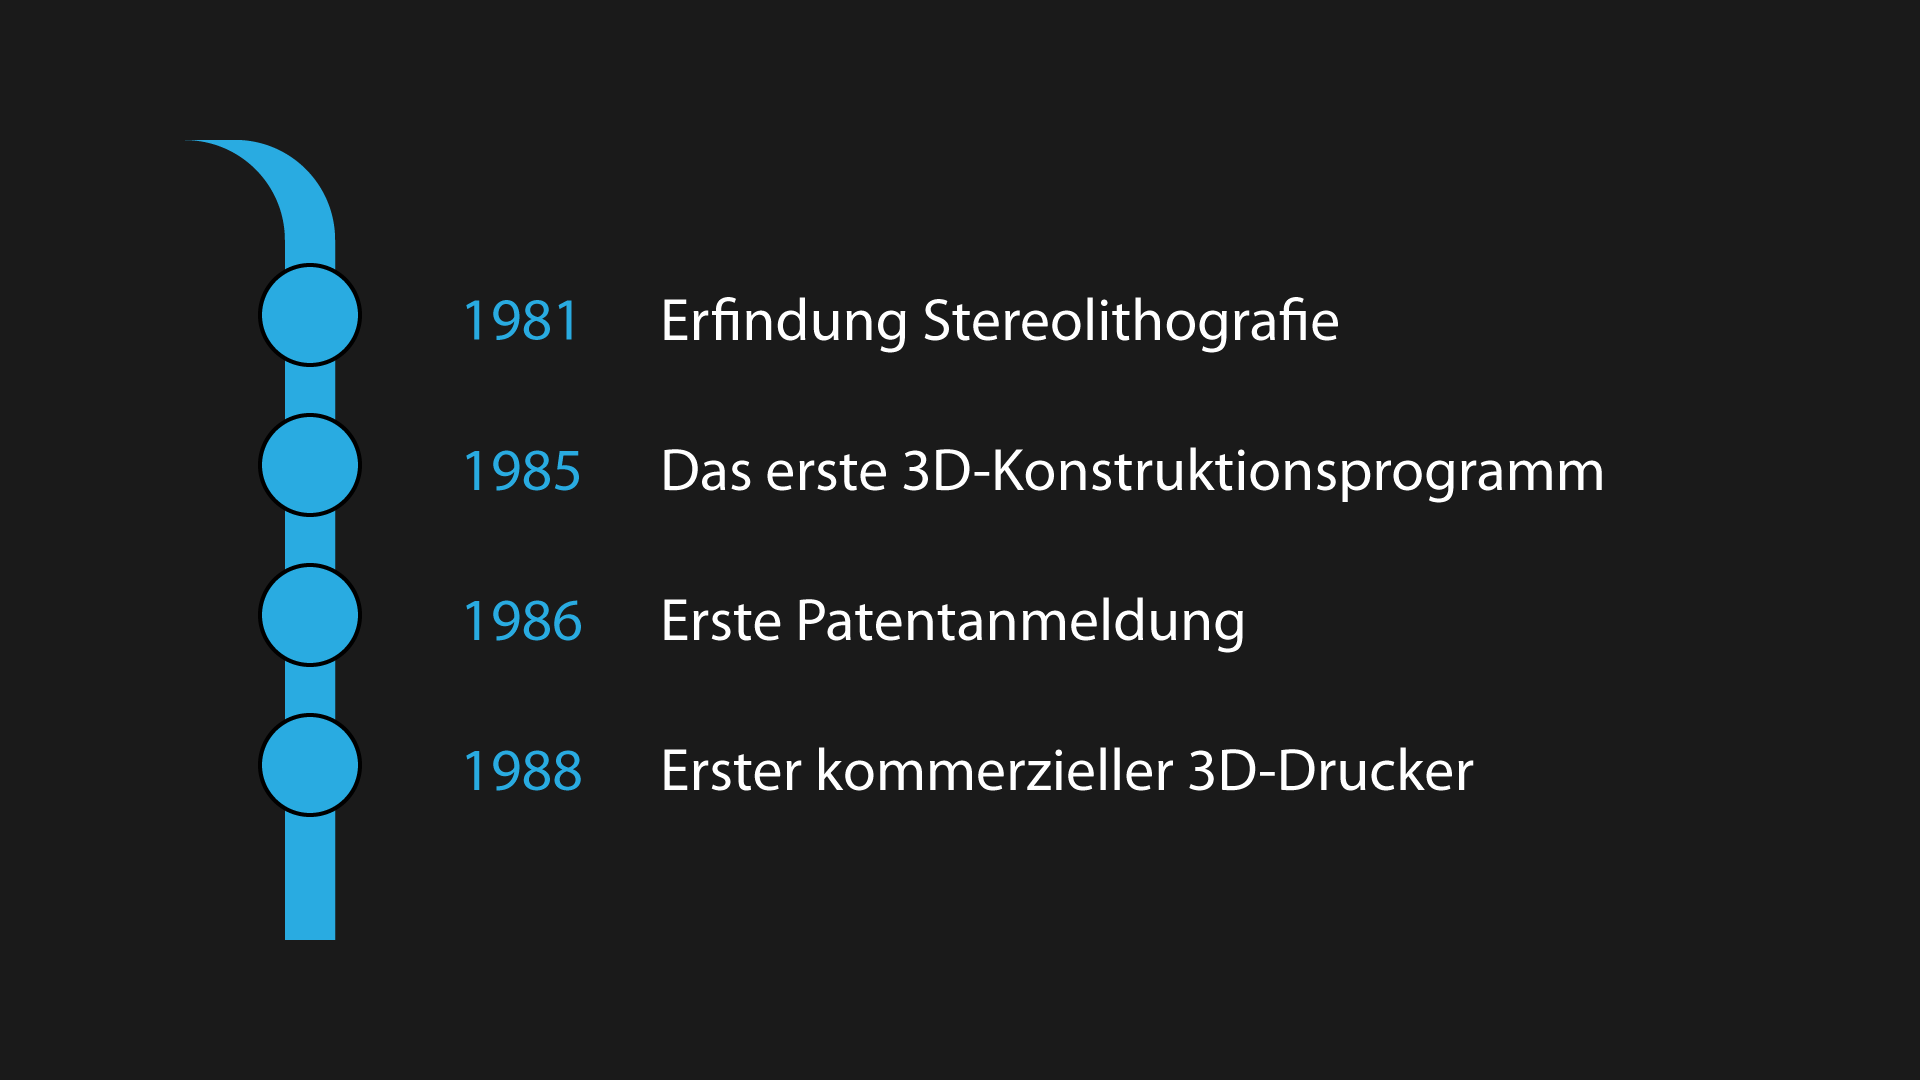
\includegraphics[width=1\paperwidth,height=1\paperheight,keepaspectratio]{images/geschichte/1980.png}};%
%\end{tikzpicture}}
\begin{frame}
  \frametitle{Seit wann gibt es 3D-Drucker}
\end{frame}
{
\usebackgroundtemplate{%
\colorbox{BackgroundJGH}{%
\vbox to \paperheight{\vfil\hbox to \paperwidth{\hfil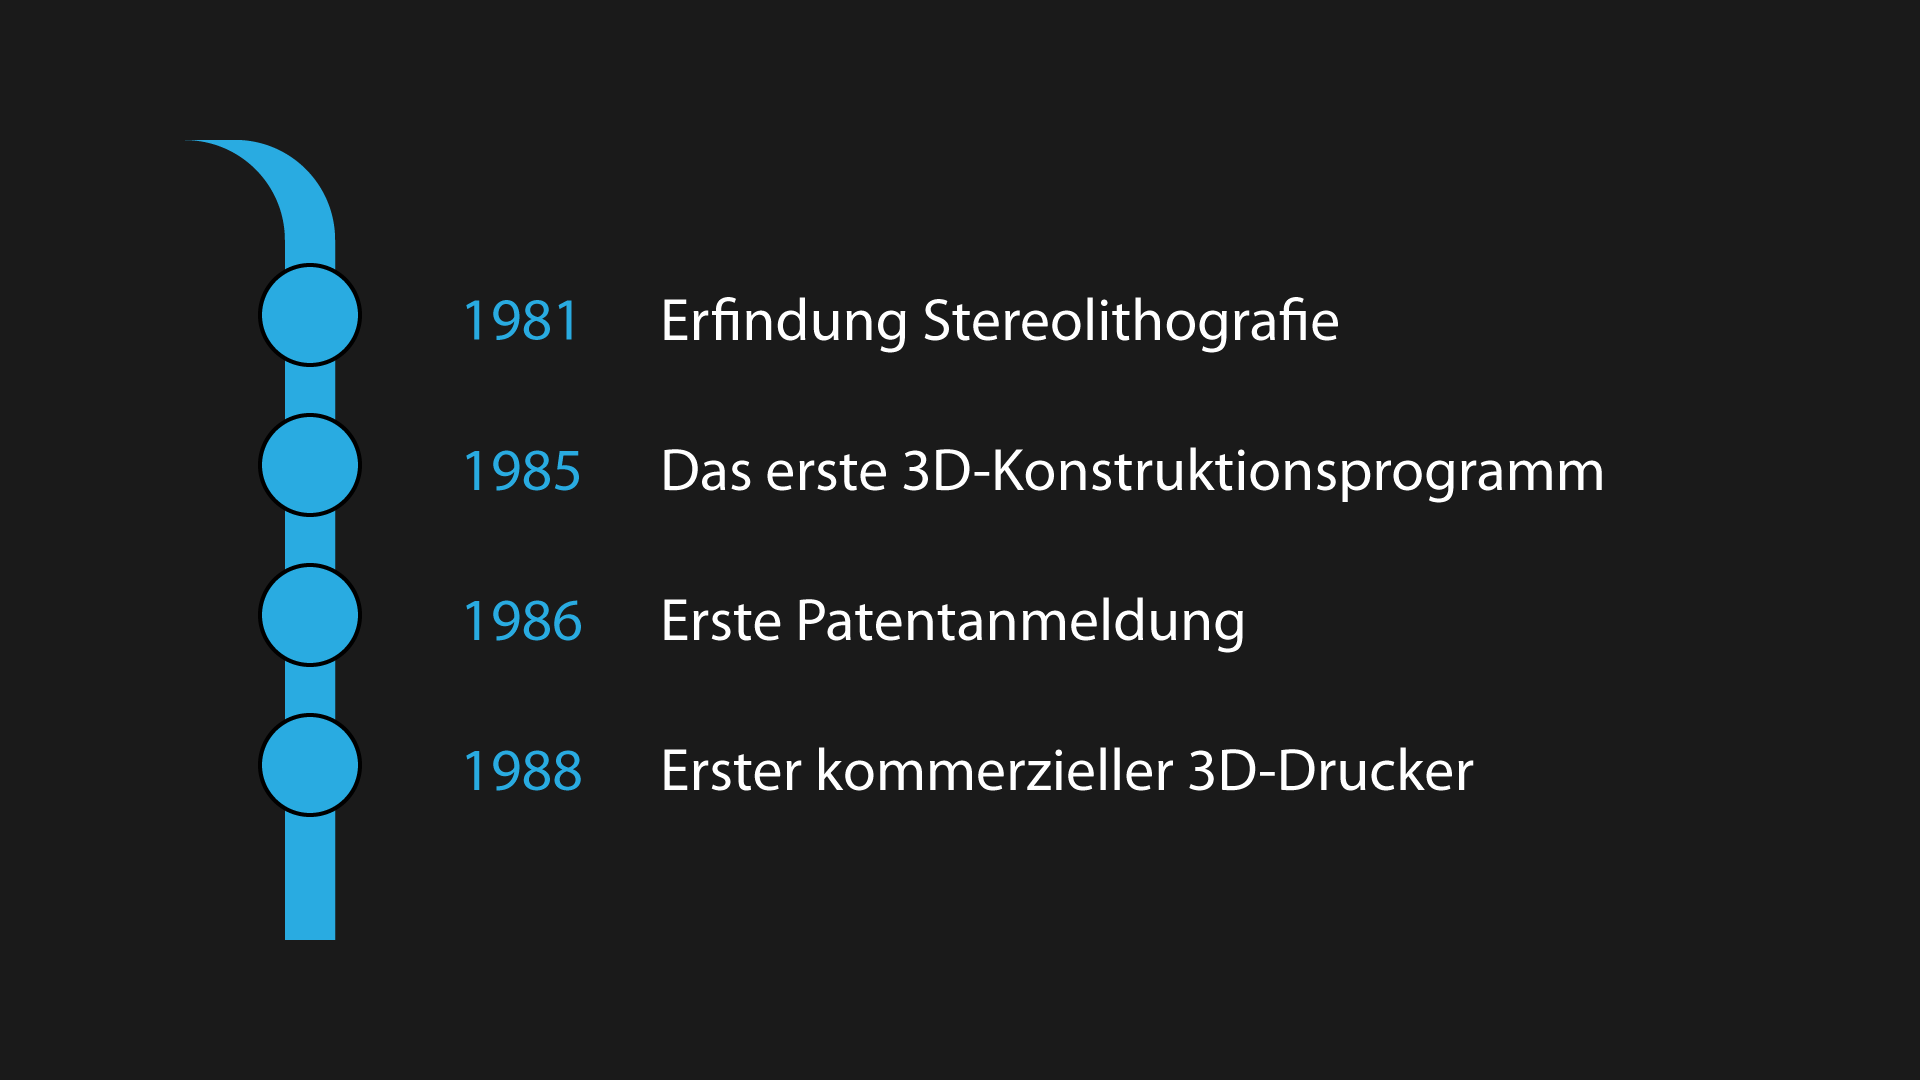
\includegraphics[width=\paperwidth]{images/geschichte/1980.png}\hfil}\vfil}
}
}
%\begin{tikzpicture}[background rectangle/.style={fill=olive!45},remember picture, overlay]%
%    \node at (current page.center) {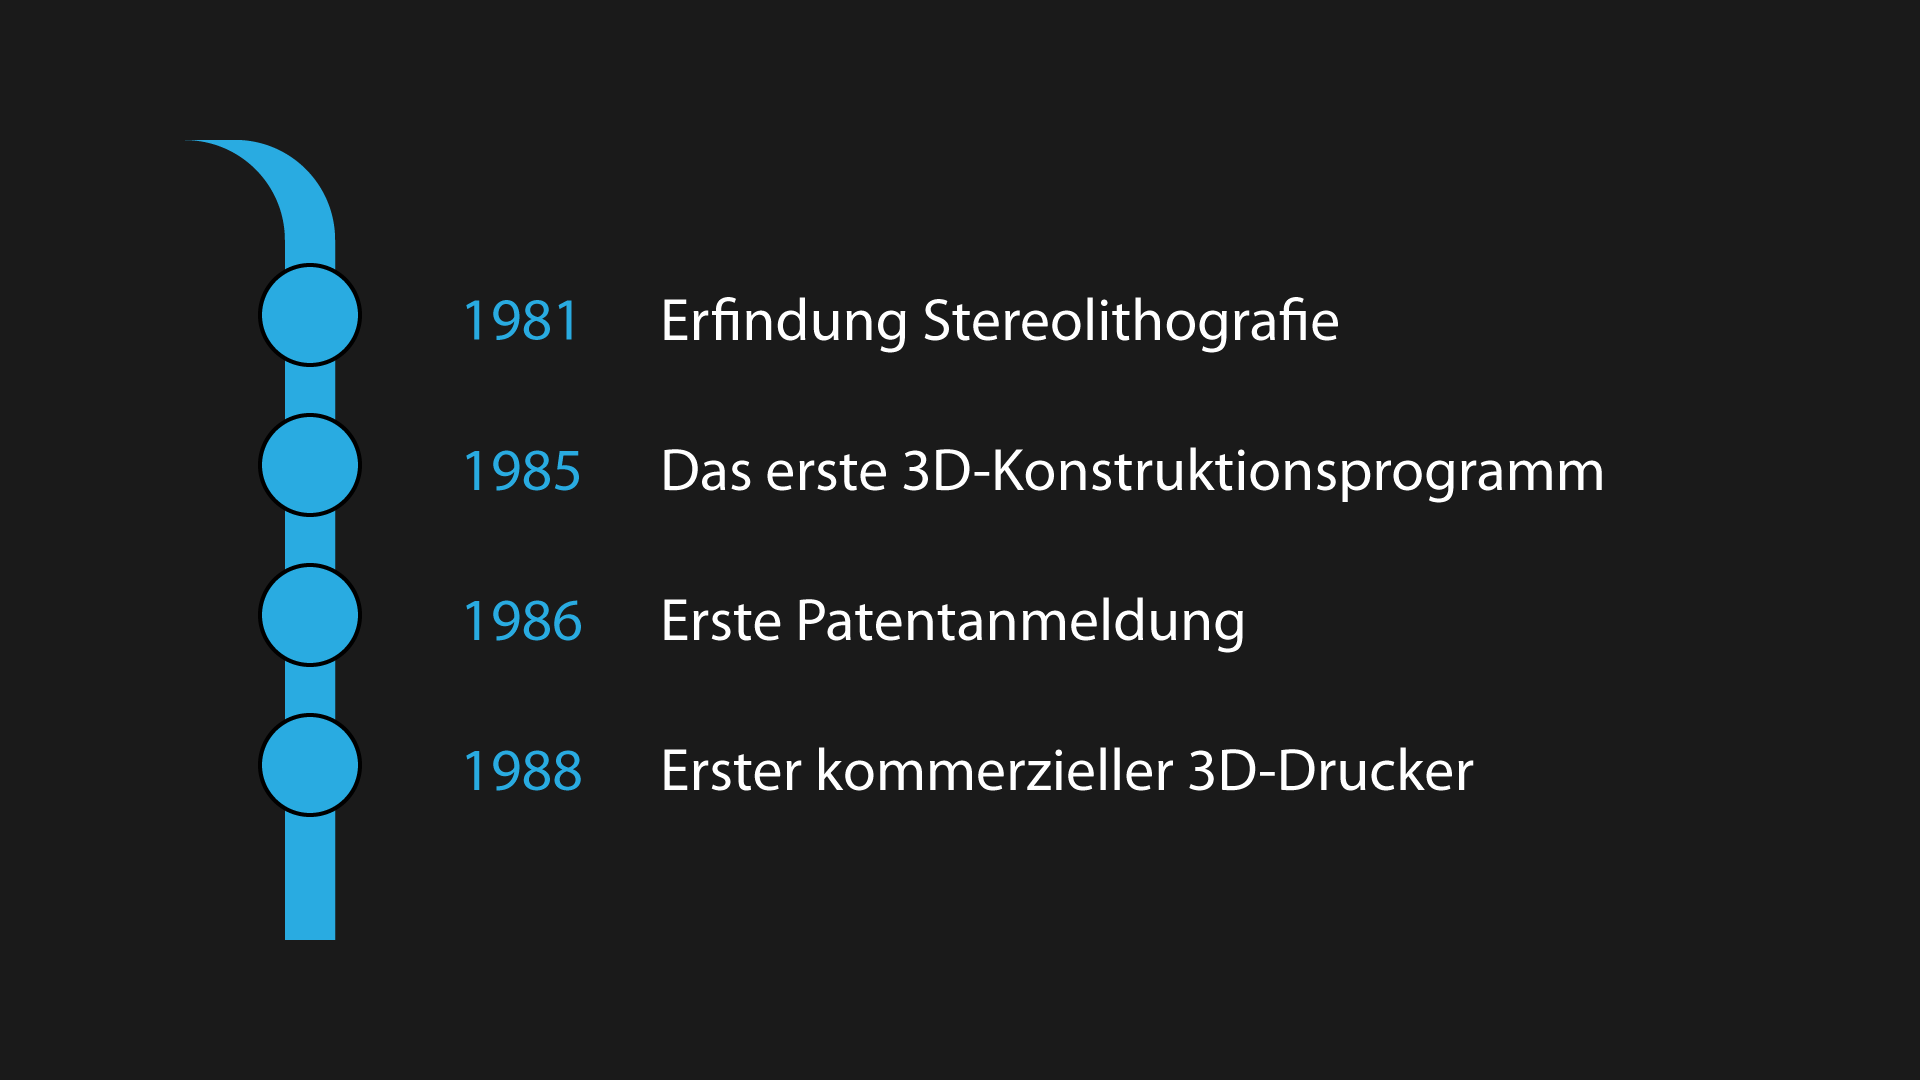
\includegraphics[width=1\paperwidth,height=1\paperheight,keepaspectratio]{images/geschichte/1980.png}};%
%\end{tikzpicture}}
\begin{frame}
  \frametitle{Seit wann gibt es 3D-Drucker}
\end{frame}
}
{
\usebackgroundtemplate{%
\colorbox{BackgroundJGH}{%
\vbox to \paperheight{\vfil\hbox to \paperwidth{\hfil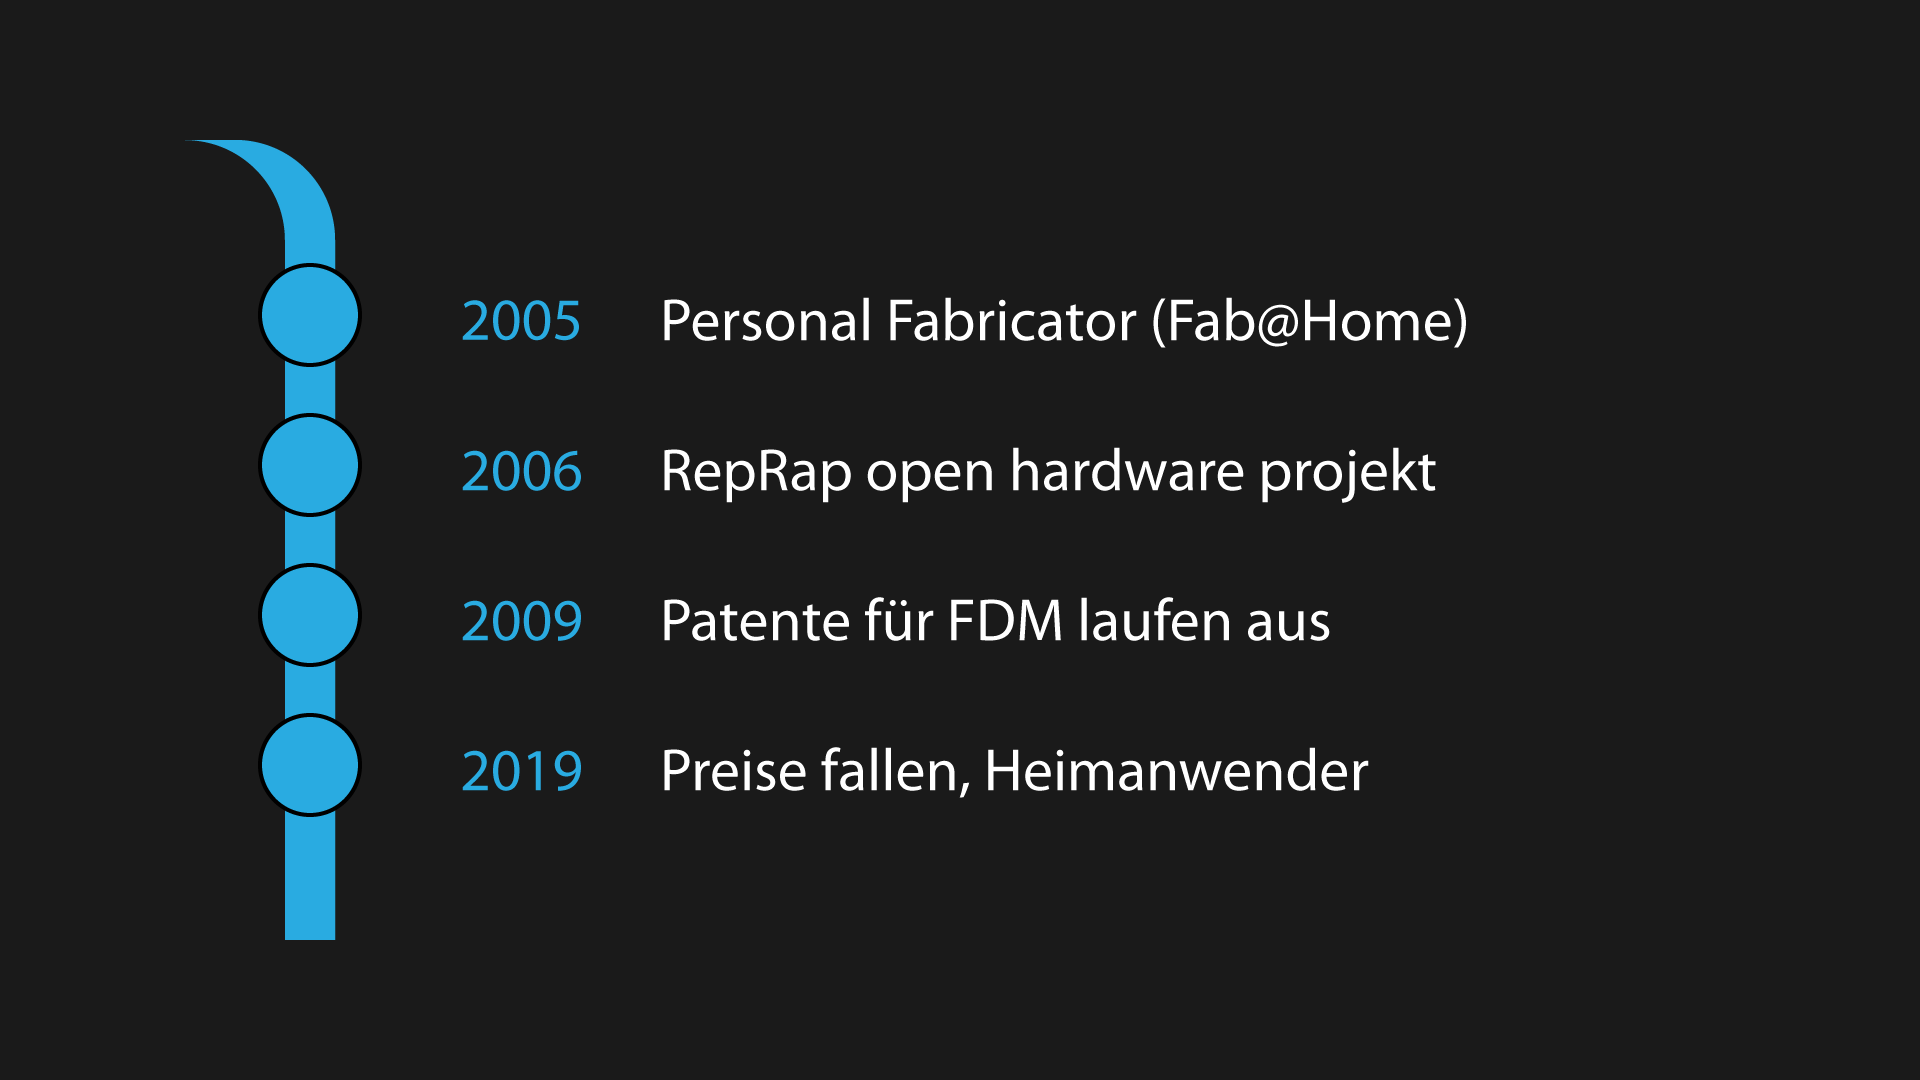
\includegraphics[width=\paperwidth]{images/geschichte/2000.png}\hfil}\vfil}
}
}
\begin{frame}
  \frametitle{Seit wann gibt es 3D-Drucker}
\end{frame}
}

\section{Welche Drucker gibt es?}
\begin{frame}
  \frametitle{Welche Drucker gibt es?}
  \pause
  \begin{itemize}
    \item \textbf{SLA} Stereolithografie \pause
    \item \textbf{SLS} Selective Laser Sintering \pause
    \item \textbf{SLM} Selective Laser Melting \pause
    \item \textbf{LOM} Laminated Object Manufacturing \pause
    \item \textbf{FDM} Fused Deposition Modeling
  \end{itemize}
\end{frame}

\begin{frame}
  \frametitle{SLA (Stereolithografie)}
  \pause
  \begin{itemize}
    \item Ältestes additives Fertigungsverfahren \pause
    \item Flüssiges Material wird mit Hilfe von UV laser ausgehärtet \pause
    \item Anwendung:
    \begin{itemize}
      \item Rapid prototyping
      \item Medizin \pause
    \end{itemize}
    \item Materialien:
    \begin{itemize}
      \item Flüssiger, lichtaushärtender Kunststoff (Photopolymer) \pause
    \end{itemize}
  \end{itemize}
  \href{https://youtu.be/8a2xNaAkvLo}{video}
\end{frame}

\begin{frame}
  \frametitle{SLS (Selective Laser Sintering)}
  \pause
  \begin{itemize}
    \item Schichtweise aufgetragenes Pulver mit Laser gesintert \pause
    \item Einsatz von Bindemitteln \pause
    \item Zu fester Schicht verschmolzen \pause
    \item Anwendung:
    \begin{itemize}
      \item Rapid prototyping
      \item Rapid tooling \pause
    \end{itemize}
    \item Materialien:
    \begin{itemize}
      \item Kunststoffpulver
      \item Metallpulver \pause
    \end{itemize}
  \end{itemize}
  \href{https://youtu.be/ruvRijM7f50}{video}
\end{frame}

\begin{frame}
  \frametitle{SLM (Selective Laser Melting)}
  \pause
  \begin{itemize}
    \item Schichtweise aufgetragenes Pulver mit Laser geschmolzen \pause
    \item Kein Einsatz von Bindemitteln \pause
    \item Zu fester Schicht verschmolzen \pause
    \item Anwendung:
    \begin{itemize}
      \item Rapid prototyping
      \item Rapid tooling \pause
    \end{itemize}
    \item Materialien:
    \begin{itemize}
      \item Kunststoffpulver
      \item Metallpulver \pause
    \end{itemize}
  \end{itemize}
  \href{https://youtu.be/yiUUZxp7bLQ}{video}
\end{frame}

\begin{frame}
  \frametitle{LOM (Laminated Object Manufacturing)}
  \pause
  \begin{itemize}
    \item Folien werden schichtweise aufgetragen, verklebt und zugeschnitten \pause
    \item Anwendung:
    \begin{itemize}
      \item Rapid prototyping \pause
    \end{itemize}
    \item Materialien:
    \begin{itemize}
      \item Papierfolien
      \item Kunststofffolien
      \item Aluminiumfolien
      \item Keramikfolien \pause
    \end{itemize}
  \end{itemize}
  \href{https://youtu.be/6C7bjzIW610}{video}
\end{frame}

\begin{frame}
  \frametitle{FDM (Fused Deposition Modeling)}
  \pause
  \begin{itemize}
    \item \textbf{FDM} ist markenrechtlich geschützt \pause
    \item Auch als \textbf{FFF} (Fused Filament Fabrication) bezeichnet. \pause
    \item Schichtweises Auftragen von geschmolzenem Filament durch heiße Düse. \pause
    \item Anwendung:
    \begin{itemize}
      \item Rapid prototyping
      \item Rapid tooling \pause
    \end{itemize}
    \item Materialien:
    \begin{itemize}
      \item Kunststoffe (thermoplaste)
    \end{itemize}
  \end{itemize}
  \href{https://youtu.be/aubLuCFIejc}{video}
\end{frame}

\section{Wie funktioniert ein Drucker?}
{
\usebackgroundtemplate{%
\colorbox{BackgroundJGH}{%
\vbox to \paperheight{\vfil\hbox to \paperwidth{\hfil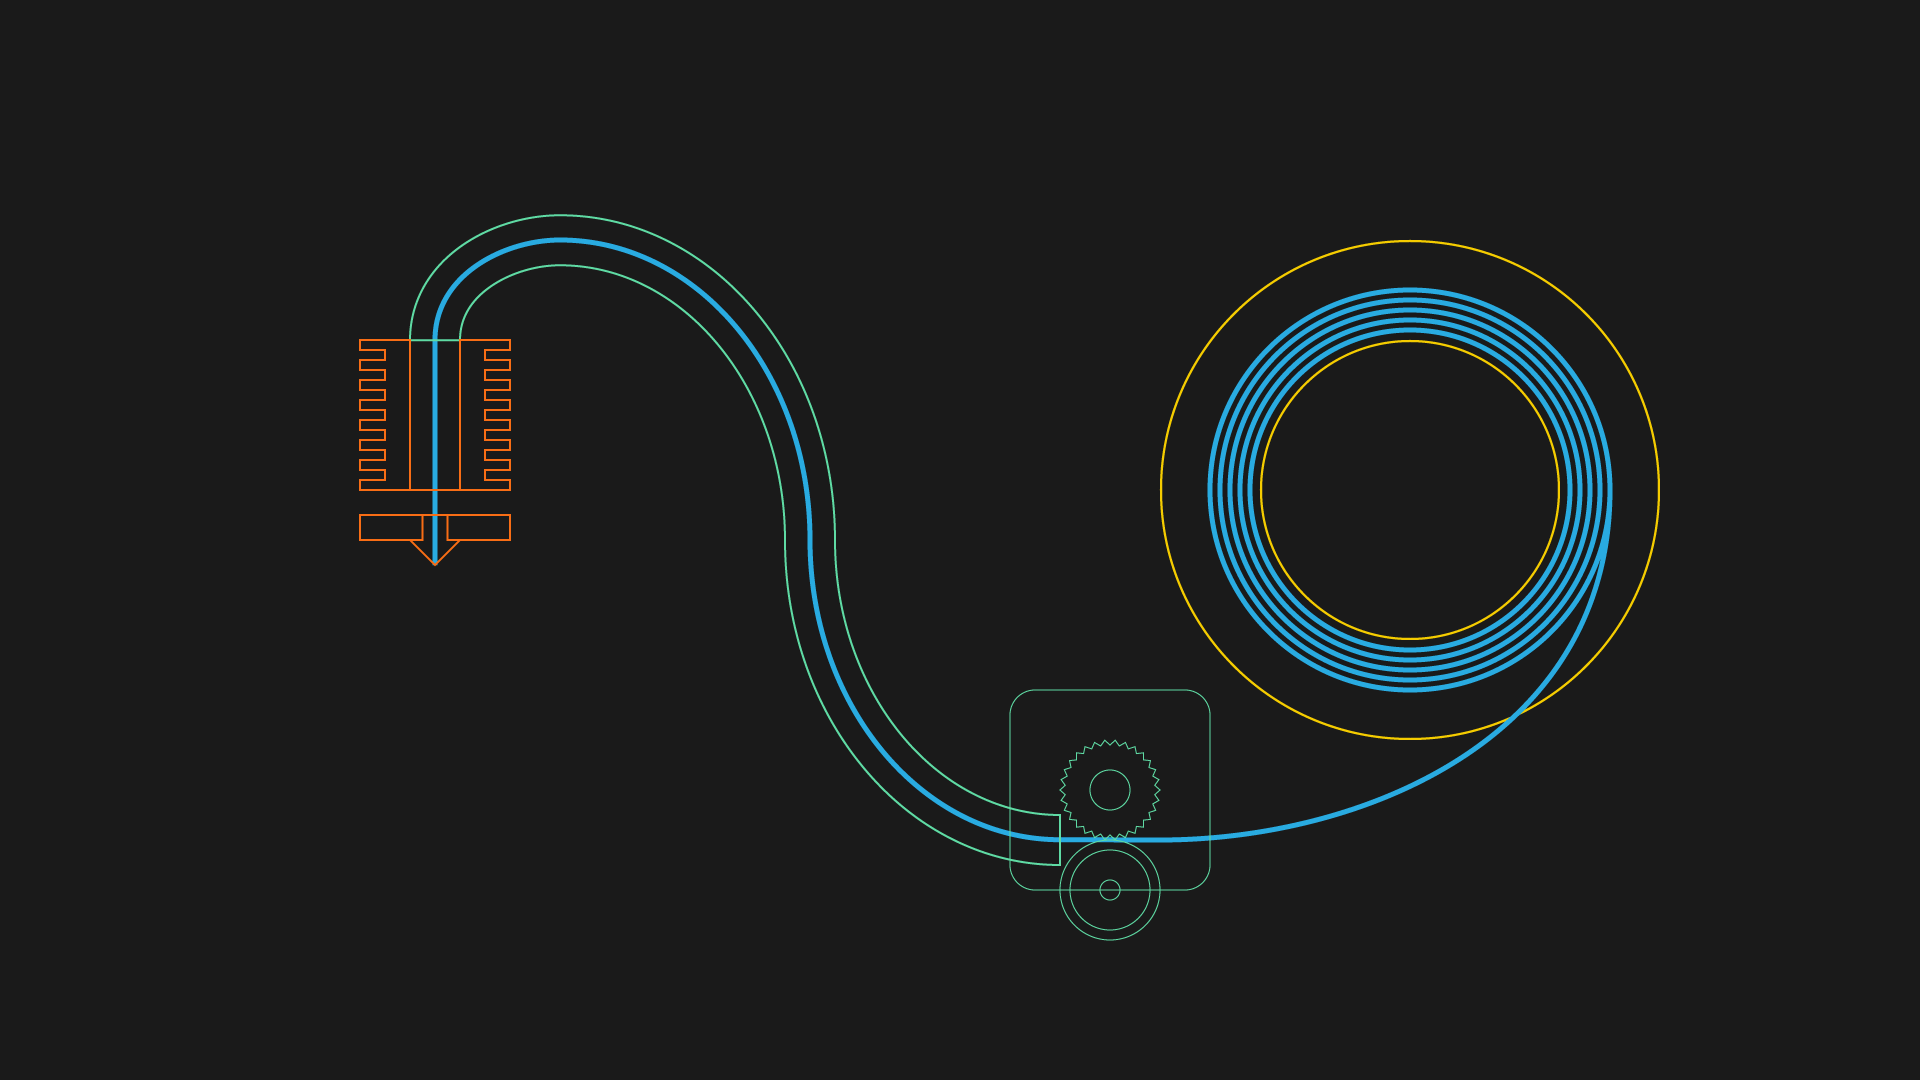
\includegraphics[width=\paperwidth]{images/extruder/bowden_drawing_colored.png}\hfil}\vfil}
}
}
\begin{frame}
  \frametitle{Wie funktioniert ein Drucker?}
\end{frame}
}
{
\usebackgroundtemplate{%
\colorbox{BackgroundJGH}{%
\vbox to \paperheight{\vfil\hbox to \paperwidth{\hfil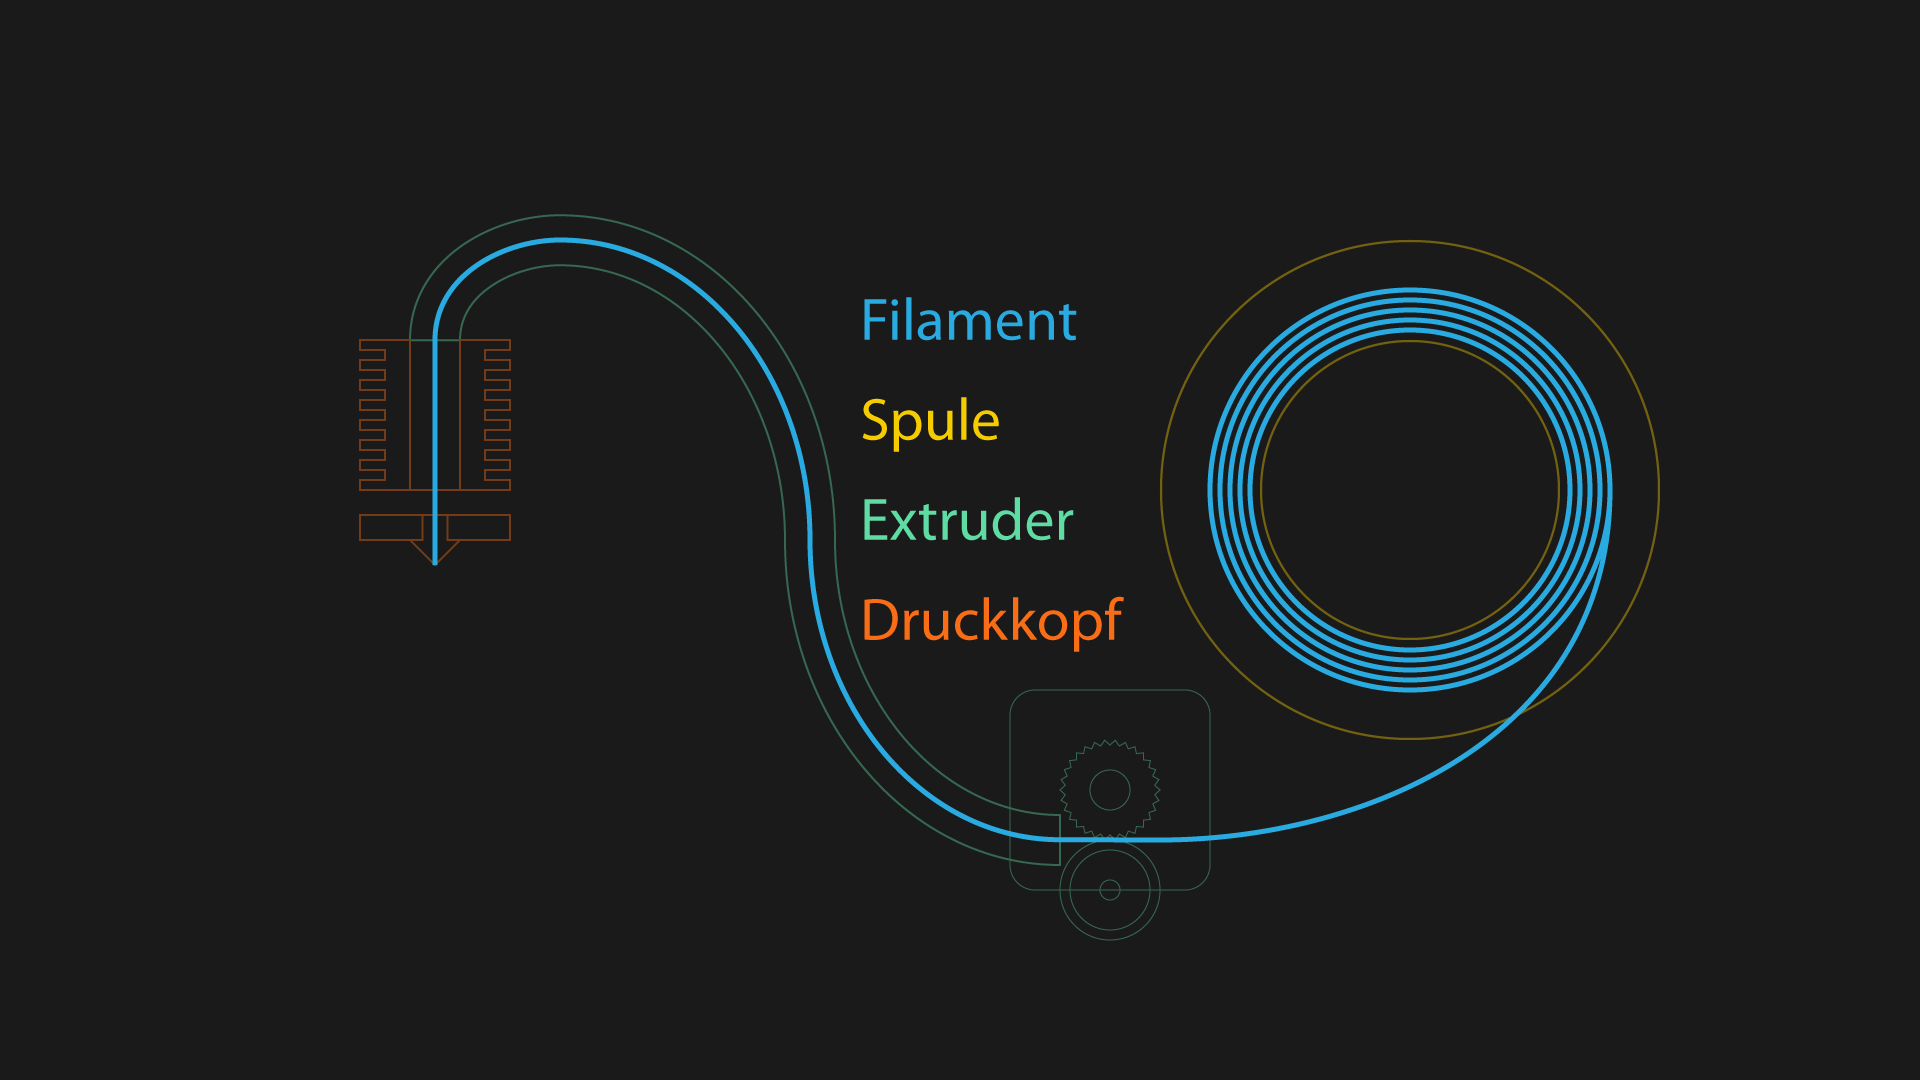
\includegraphics[width=\paperwidth]{images/extruder/filament_flow.png}\hfil}\vfil}
}
}
\subsection{Wie funktioniert das mit dem Filament?}
\begin{frame}
  \frametitle{Wie funktioniert das mit dem Filament?}
\end{frame}
}


\usebackgroundtemplate{%
\colorbox{BackgroundJGH}{%
\vbox to \paperheight{\vfil\hbox to \paperwidth{\hfil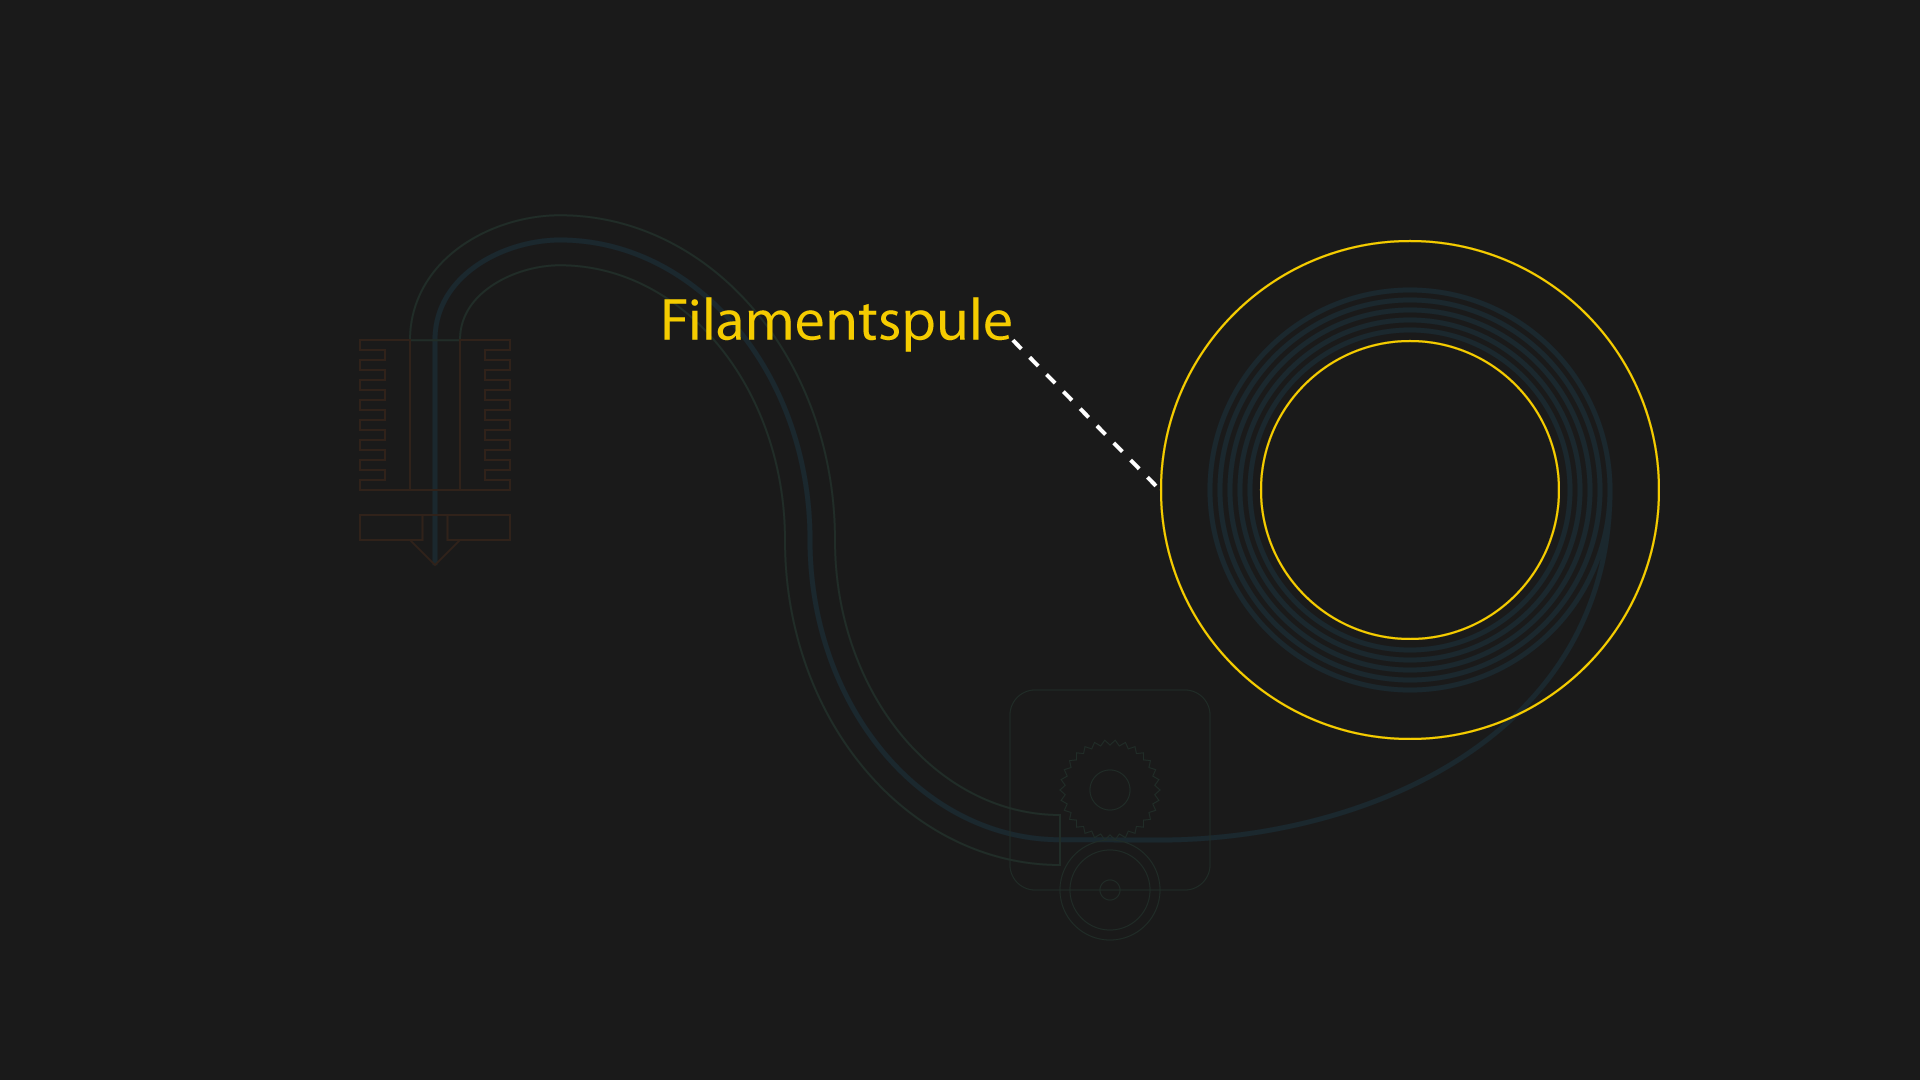
\includegraphics[width=\paperwidth]{images/extruder/filament_spool.png}\hfil}\vfil}
}
\begin{frame}
  \frametitle{Filamentspule}
\end{frame}
}
{
\usebackgroundtemplate{%
\colorbox{BackgroundJGH}{%
\vbox to \paperheight{\vfil\hbox to \paperwidth{\hfil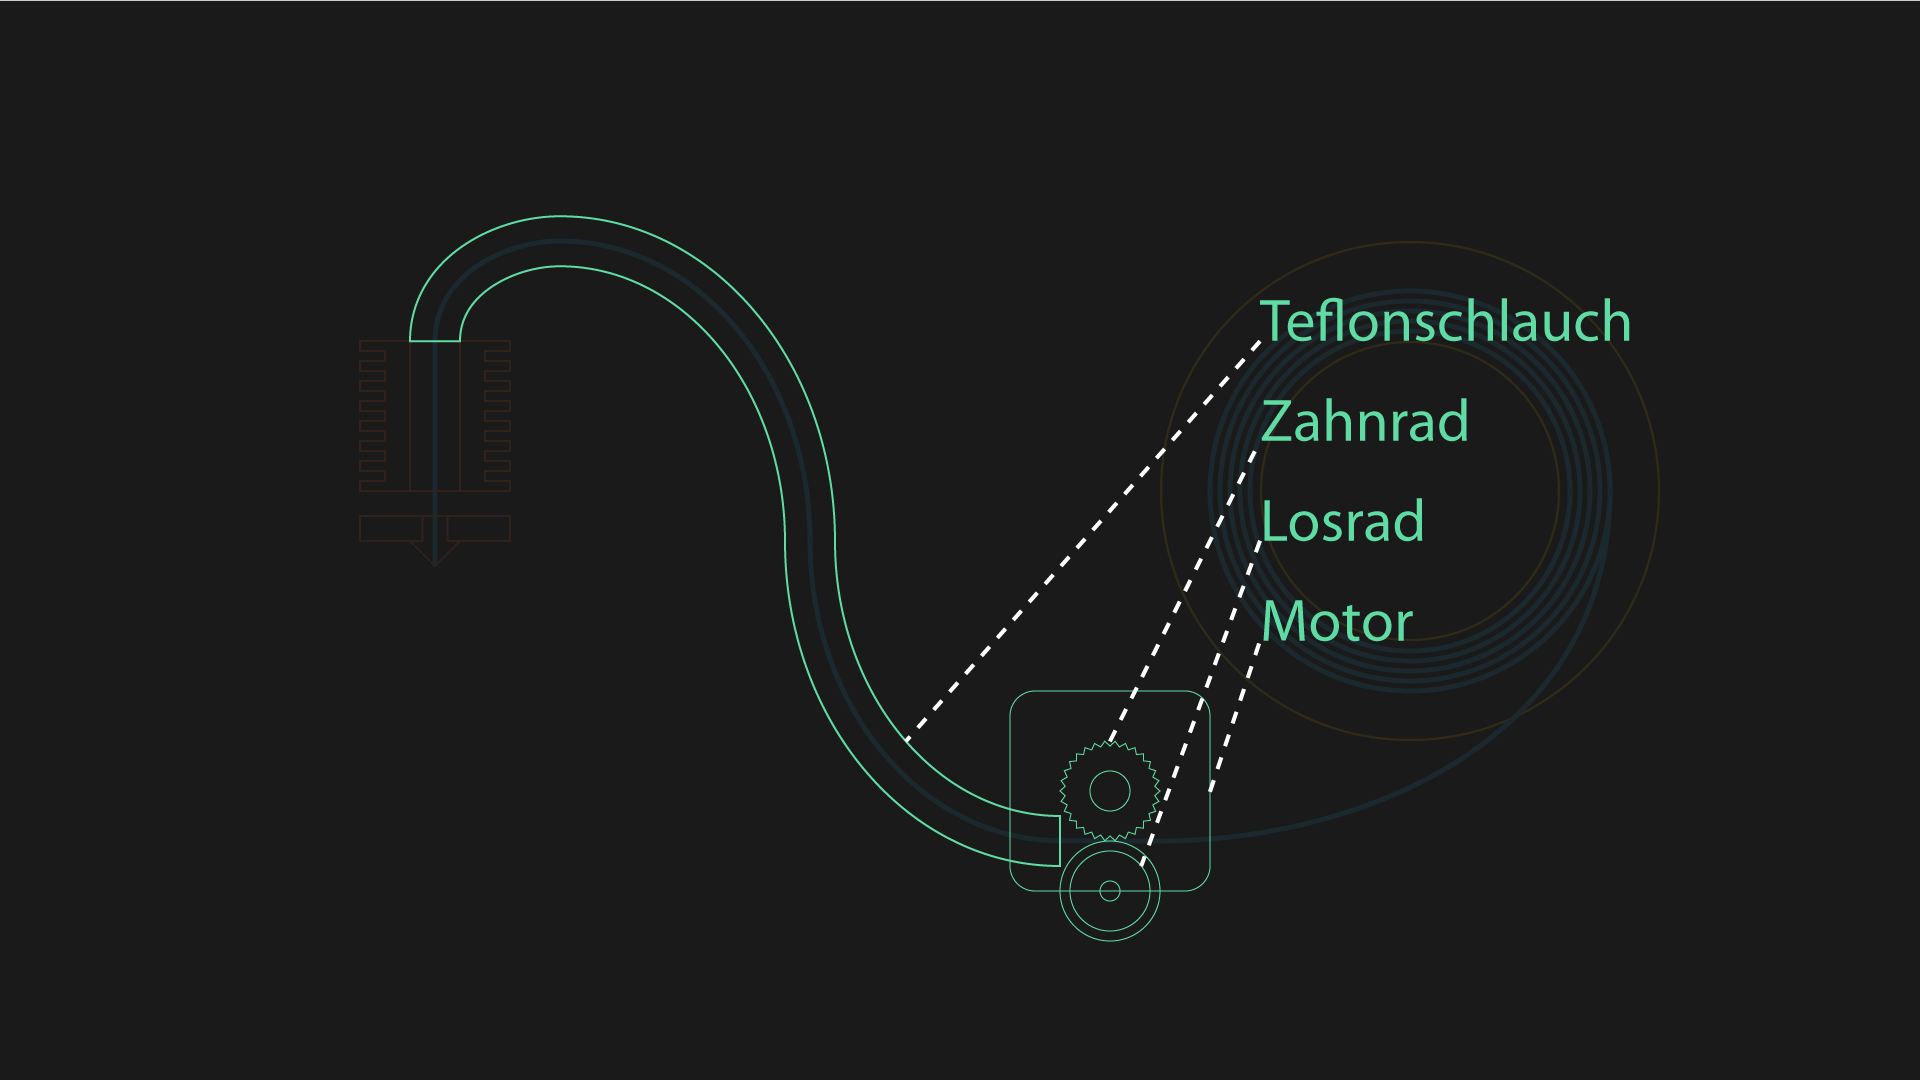
\includegraphics[width=\paperwidth]{images/extruder/bowden.png}\hfil}\vfil}
}
}
\begin{frame}
  \frametitle{Bowden Extruder}
\end{frame}
}
{
\usebackgroundtemplate{%
\colorbox{BackgroundJGH}{%
\vbox to \paperheight{\vfil\hbox to \paperwidth{\hfil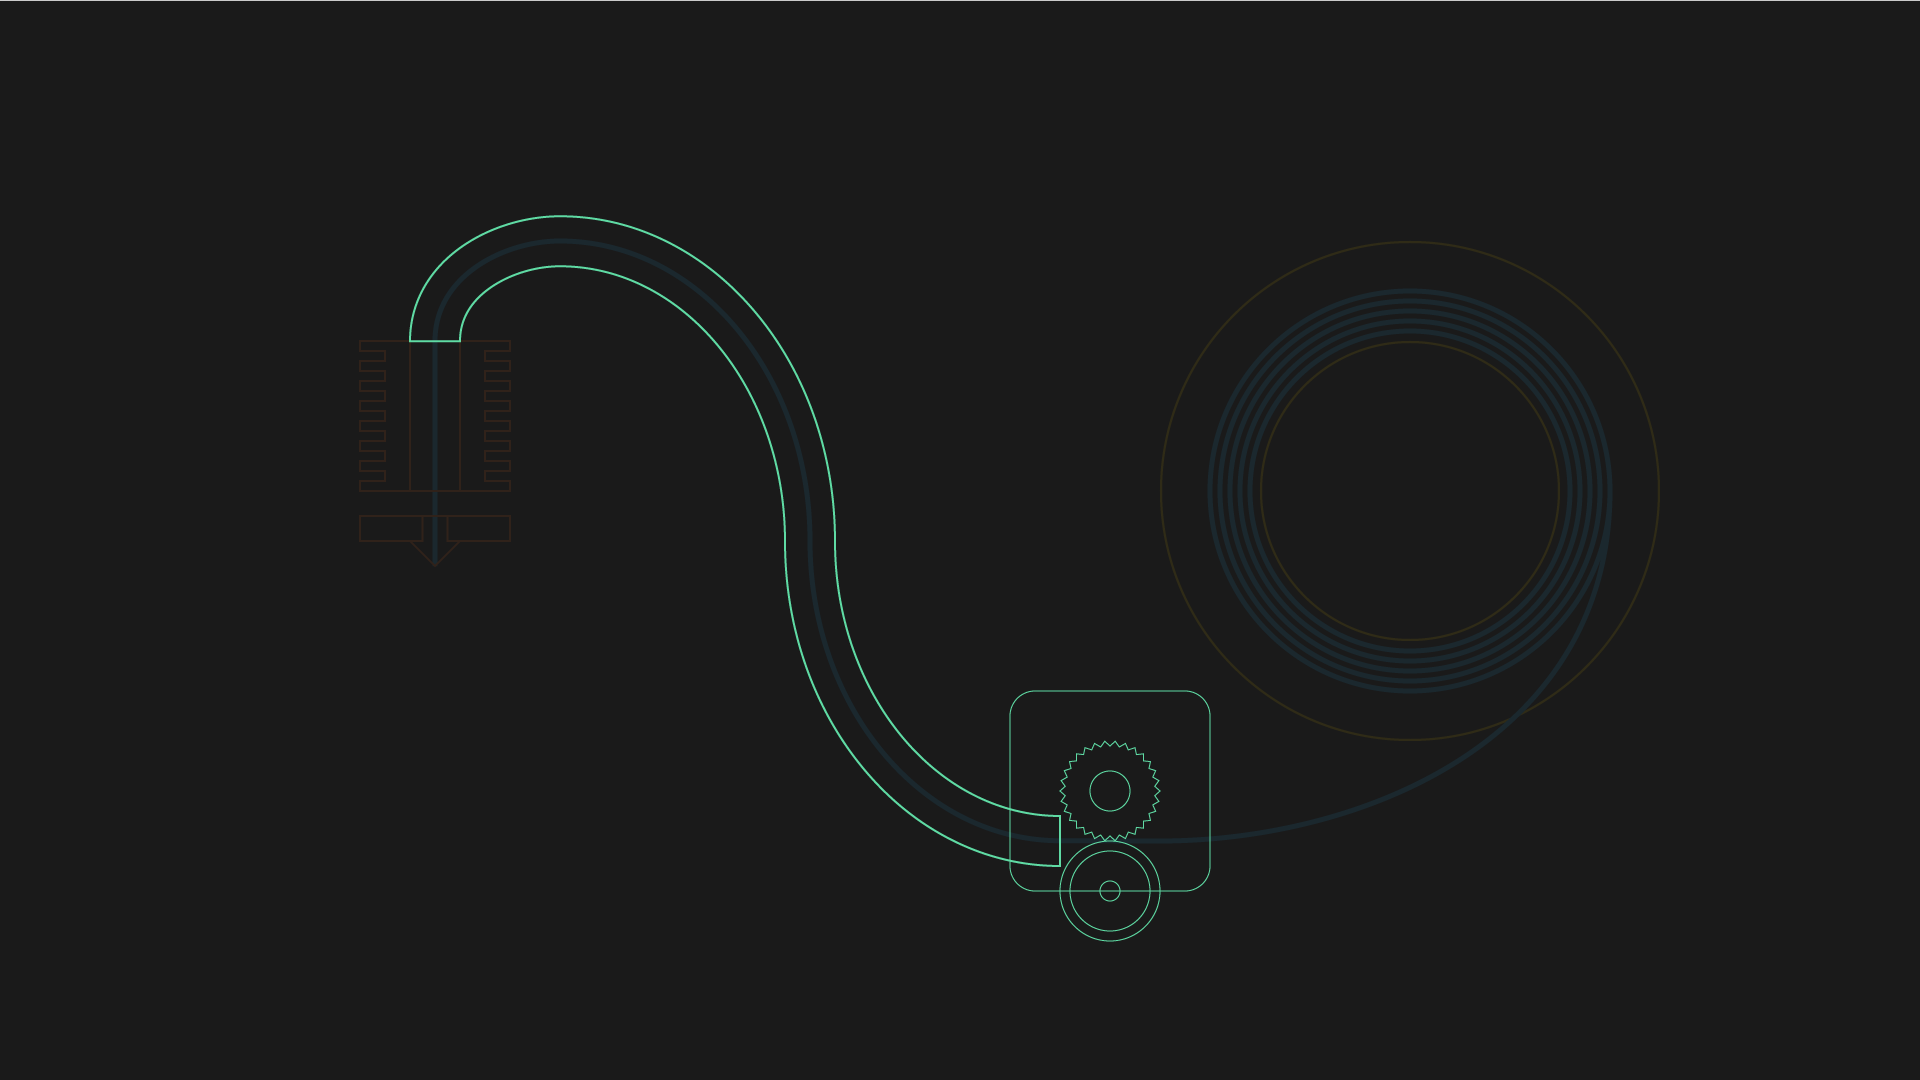
\includegraphics[width=\paperwidth]{images/extruder/bowden_no_text.png}\hfil}\vfil}
}
}
\begin{frame}
  \frametitle{Bowden Extruder}
  \pause
  \begin{itemize}
    \item Leicht zu tauschen \pause
    \item Weniger Masse am Druckkopf
    \begin{itemize}
      \item Schnellere Bewegungen
      \item Schnellere Druckgeschwindigkeit
      \item Höhere Genauigkeit \pause
    \end{itemize}
    \item Langer Bowdentube
    \begin{itemize}
      \item Reibung
      \item Dehnung/Stauchung des Filaments
    \end{itemize}
  \end{itemize}
\end{frame}
}
{
\usebackgroundtemplate{%
\colorbox{BackgroundJGH}{%
\vbox to \paperheight{\vfil\hbox to \paperwidth{\hfil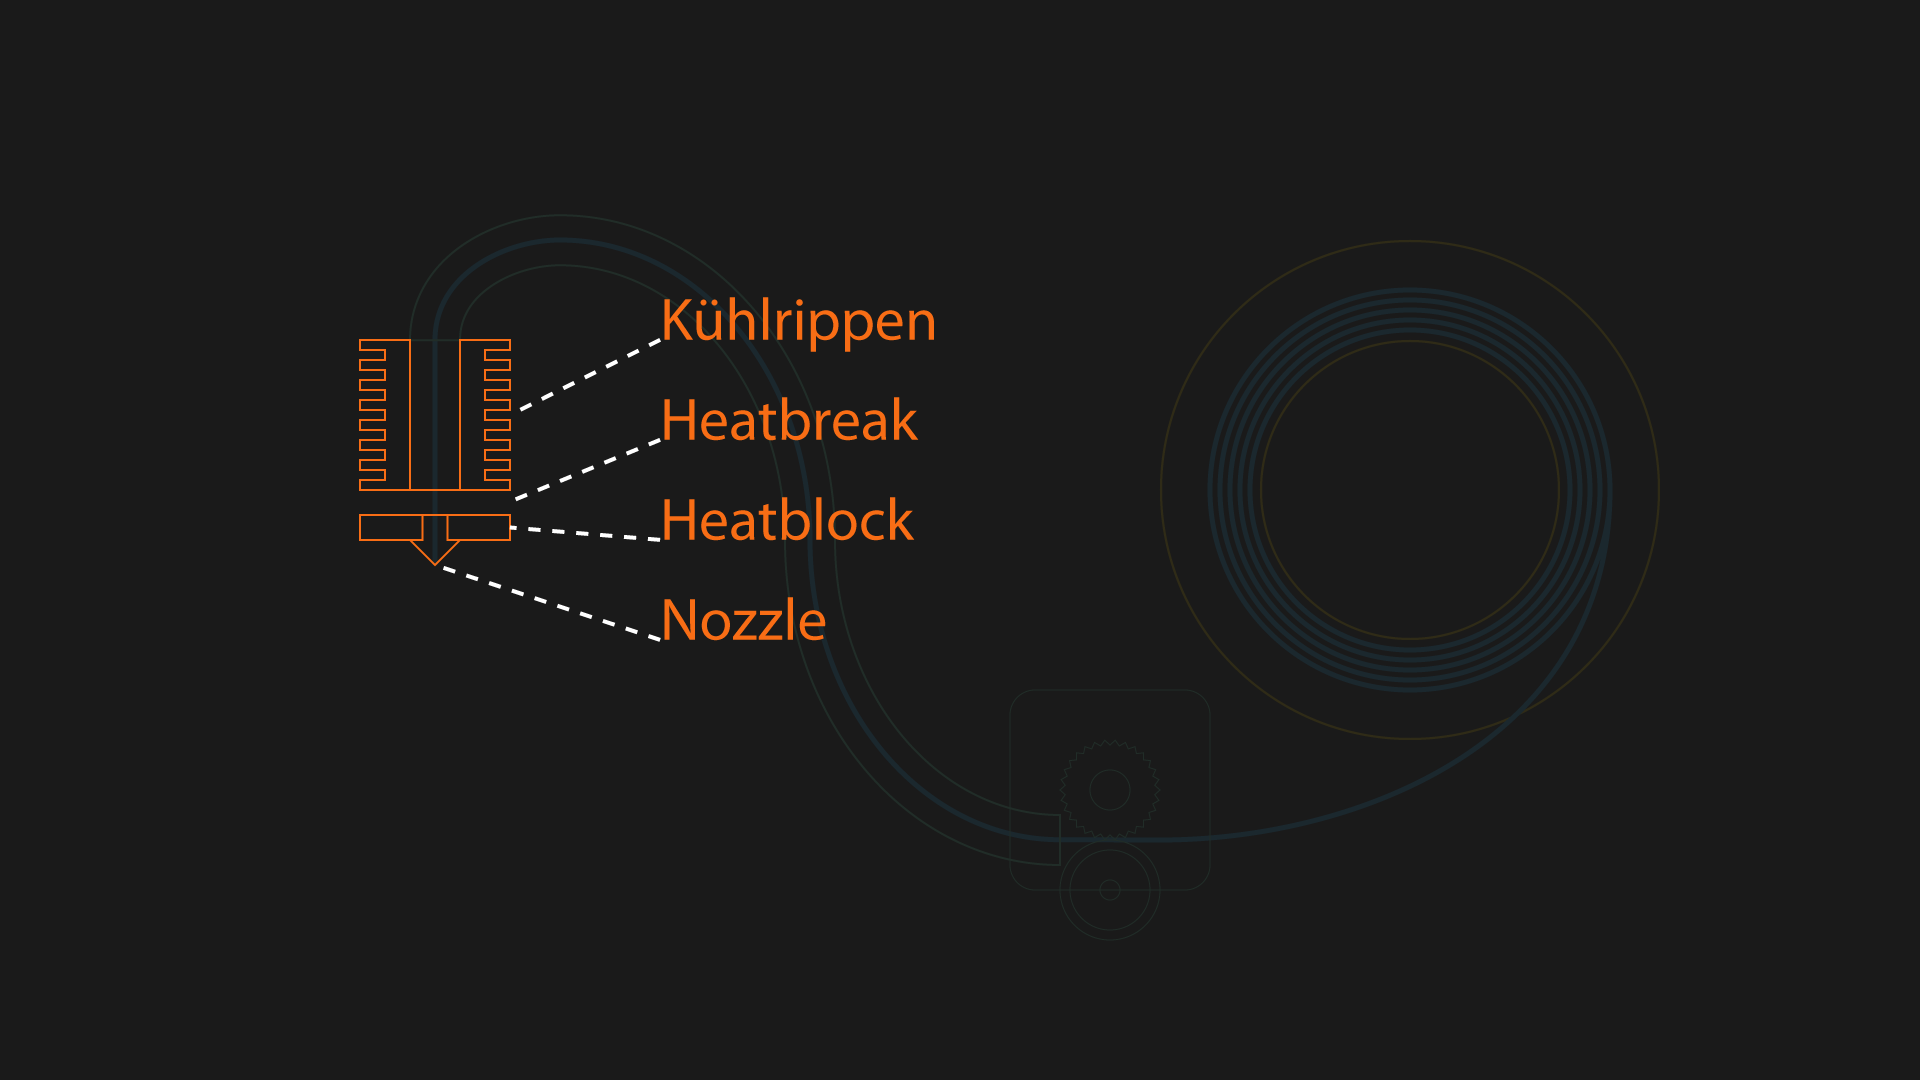
\includegraphics[width=\paperwidth]{images/extruder/print_head.png}\hfil}\vfil}
}
}
\begin{frame}
  \frametitle{Druckkopf}
\end{frame}
}
{
\usebackgroundtemplate{%
\colorbox{BackgroundJGH}{%
\vbox to \paperheight{\vfil\hbox to \paperwidth{\hfil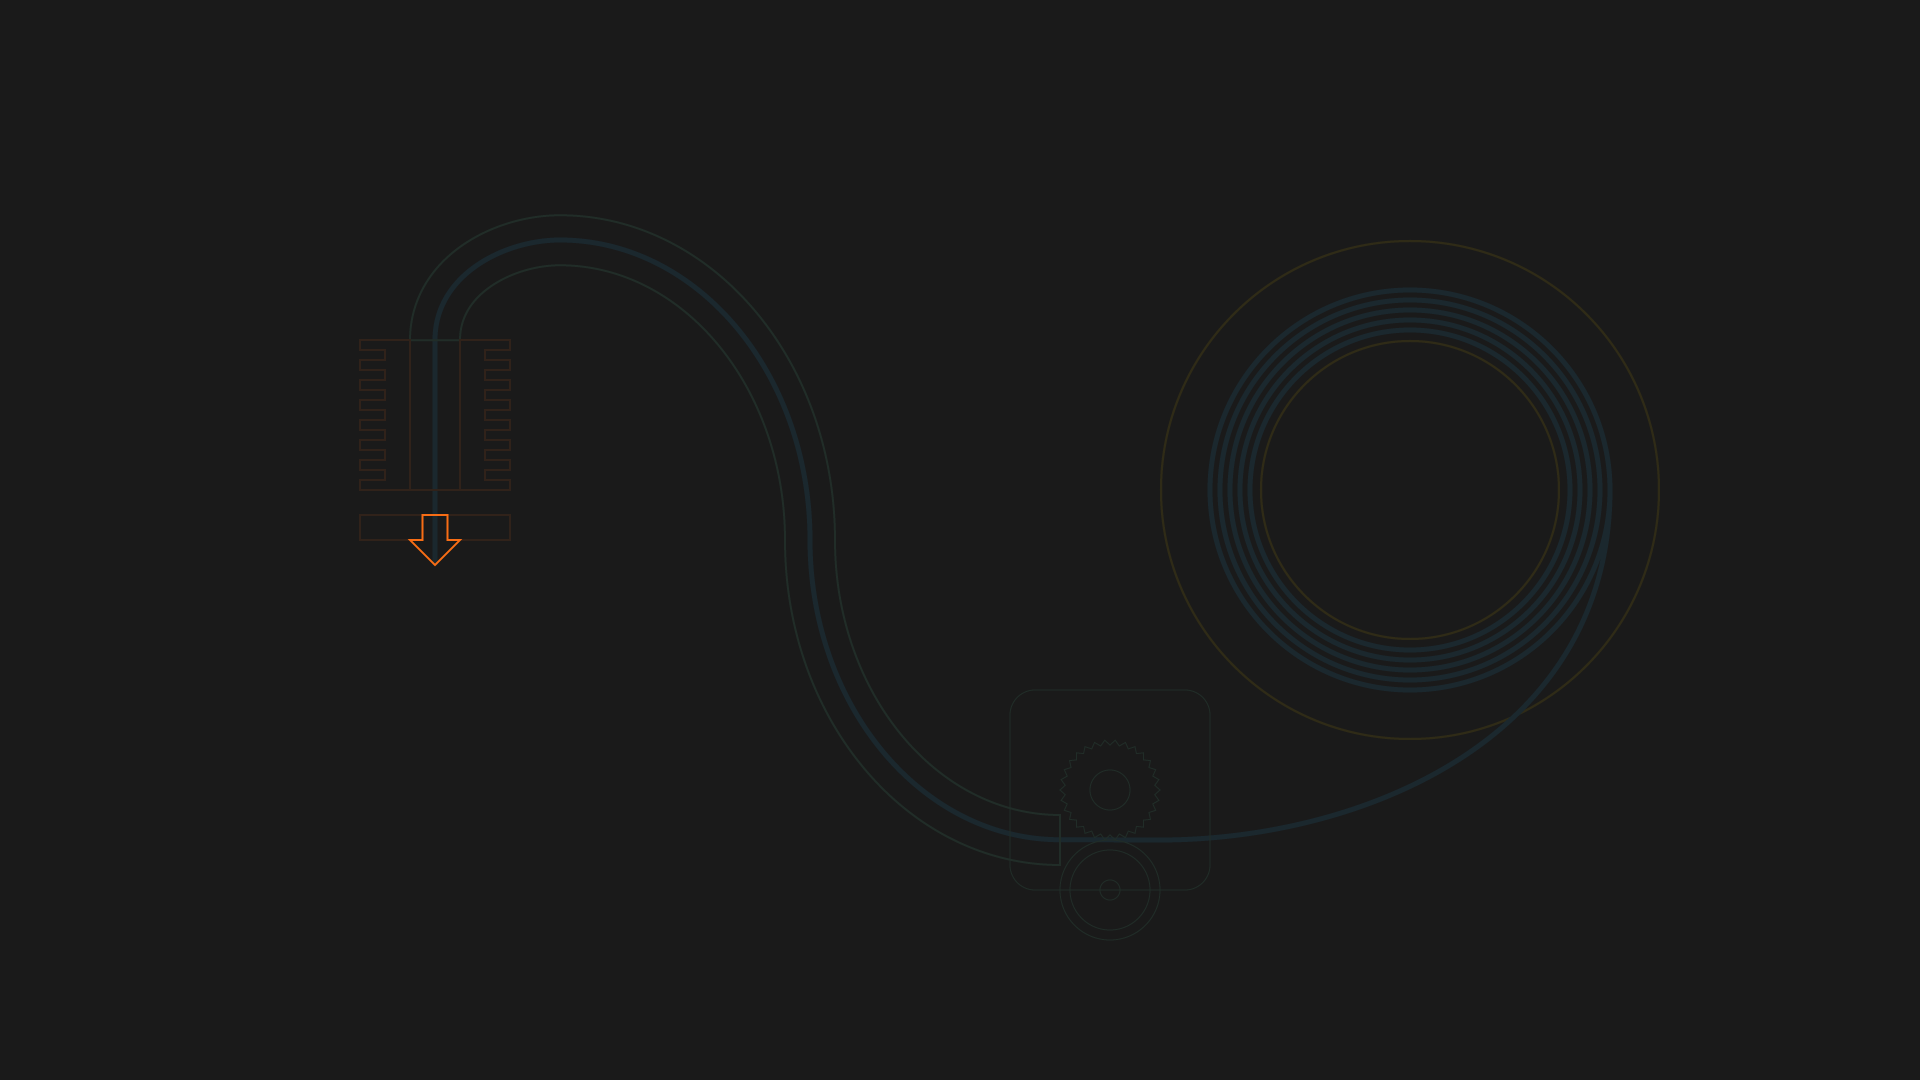
\includegraphics[width=\paperwidth]{images/extruder/nozzle.png}\hfil}\vfil}
}
}
\begin{frame}
  \frametitle{Nozzle}
  \pause
  \begin{itemize}
    \item Wird nach der Größe der Öffnung benannt \pause
    \item Meist 0.4mm Durchmesser \pause
    \item Gibt Schichtdicke und Wandbreite vor \pause
    \begin{itemize}
      \item 0.4mm ermöglicht 0.1-0.3mm Schichtdicke
      \item Wandstärke immer ein Vielfaches des Nozzledurchmessers
      \item Höhen immer ein Vielfaches der Schichtdicke
    \end{itemize}
  \end{itemize}
\end{frame}
}

\subsection{Wie wird der Druckkopf bewegt?}
{
\usebackgroundtemplate{%
\colorbox{BackgroundJGH}{%
\vbox to \paperheight{\vfil\hbox to \paperwidth{\hfil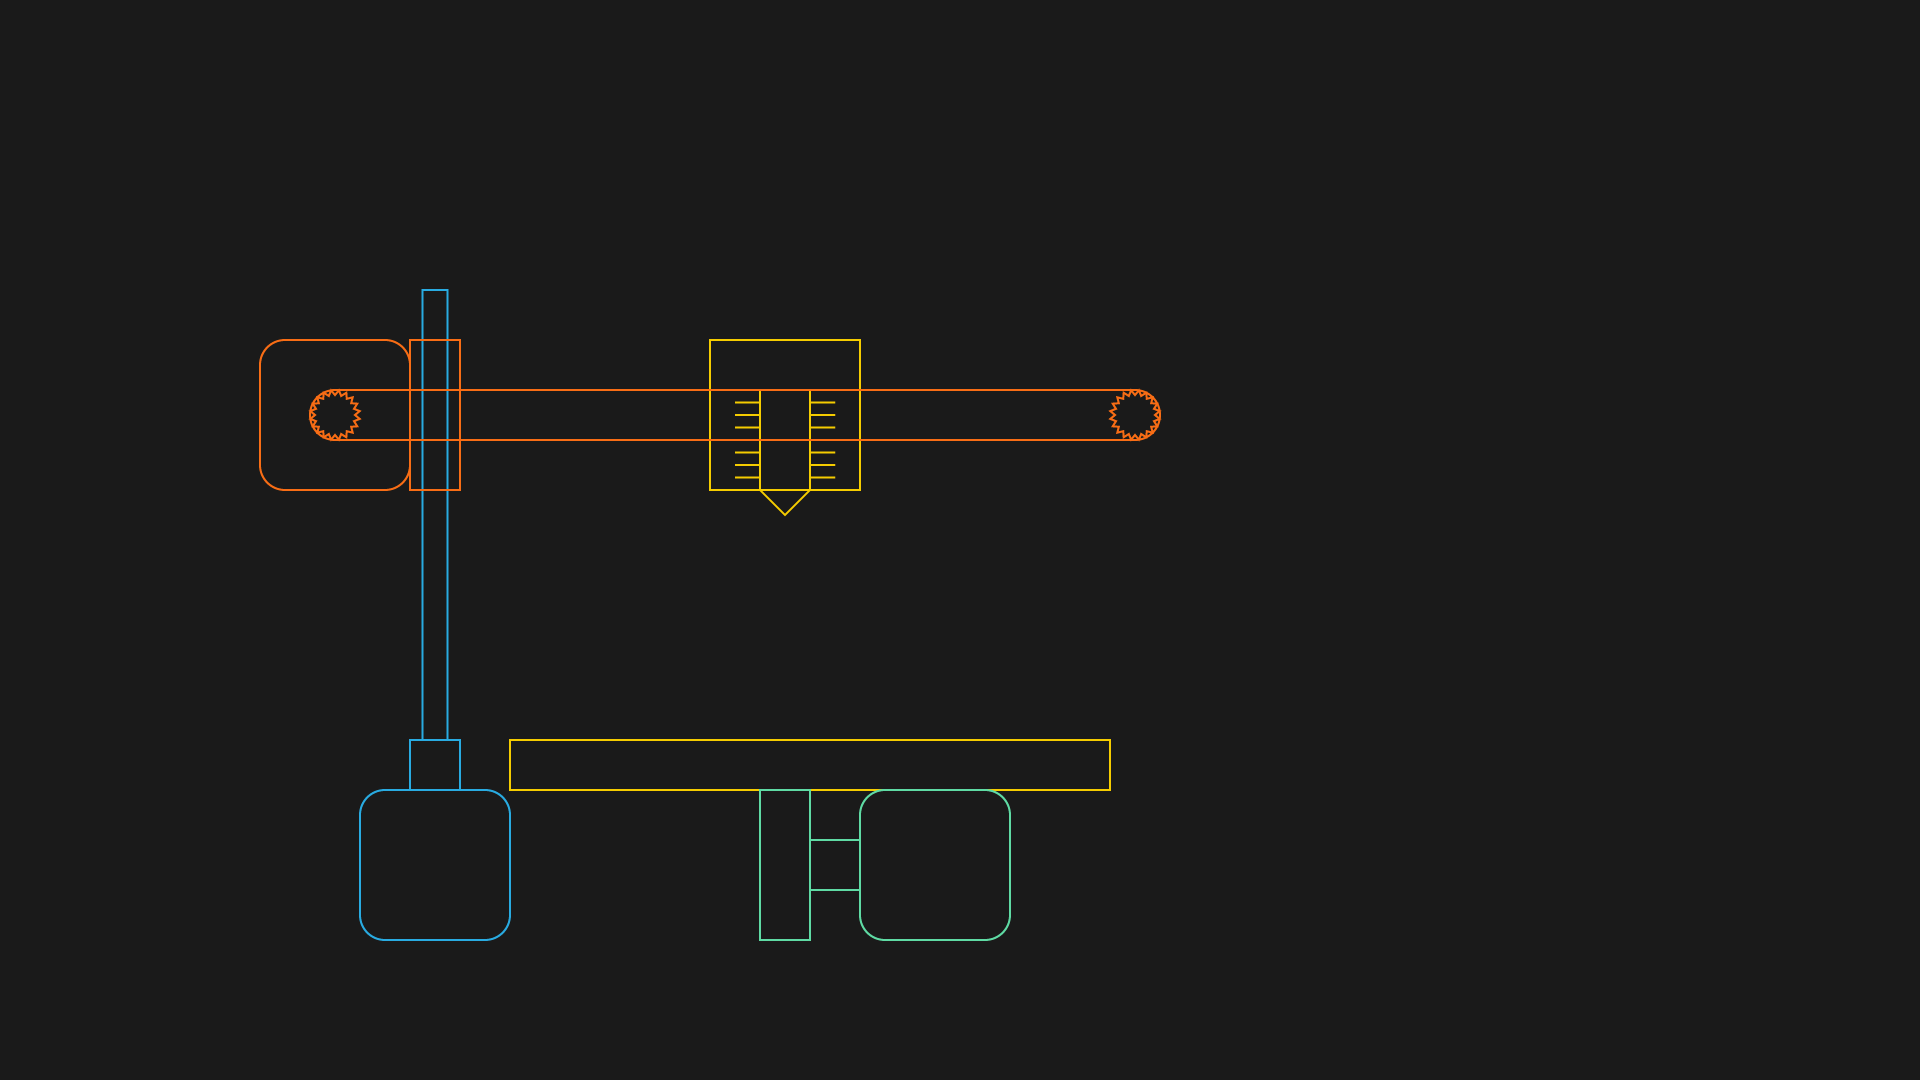
\includegraphics[width=\paperwidth]{images/mechanik/complete.png}\hfil}\vfil}
}
}
\begin{frame}
  \frametitle{Wie wird der Druckkopf bewegt?}
\end{frame}
}

{
\usebackgroundtemplate{%
\colorbox{BackgroundJGH}{%
\vbox to \paperheight{\vfil\hbox to \paperwidth{\hfil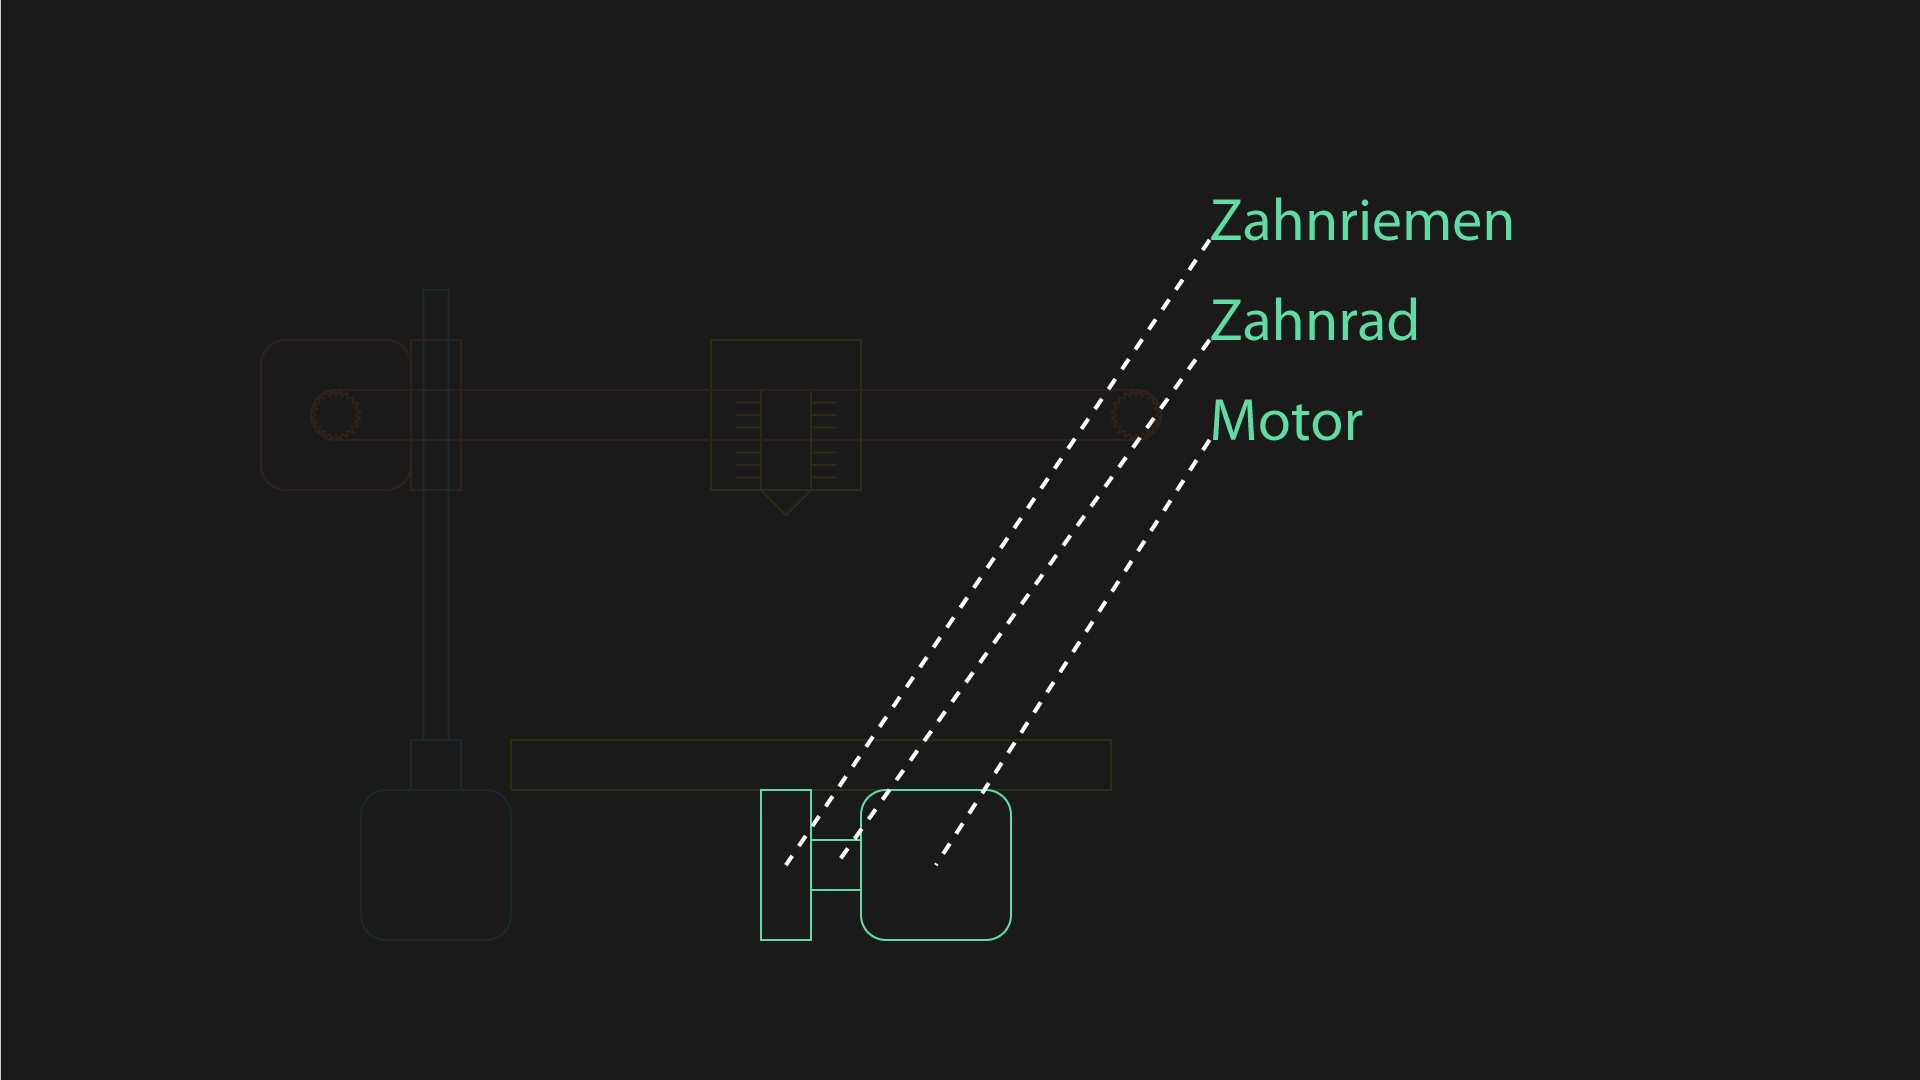
\includegraphics[width=\paperwidth]{images/mechanik/y-axis.png}\hfil}\vfil}
}
}
\begin{frame}
  \frametitle{Y-Achse}
\end{frame}
}

{
\usebackgroundtemplate{%
\colorbox{BackgroundJGH}{%
\vbox to \paperheight{\vfil\hbox to \paperwidth{\hfil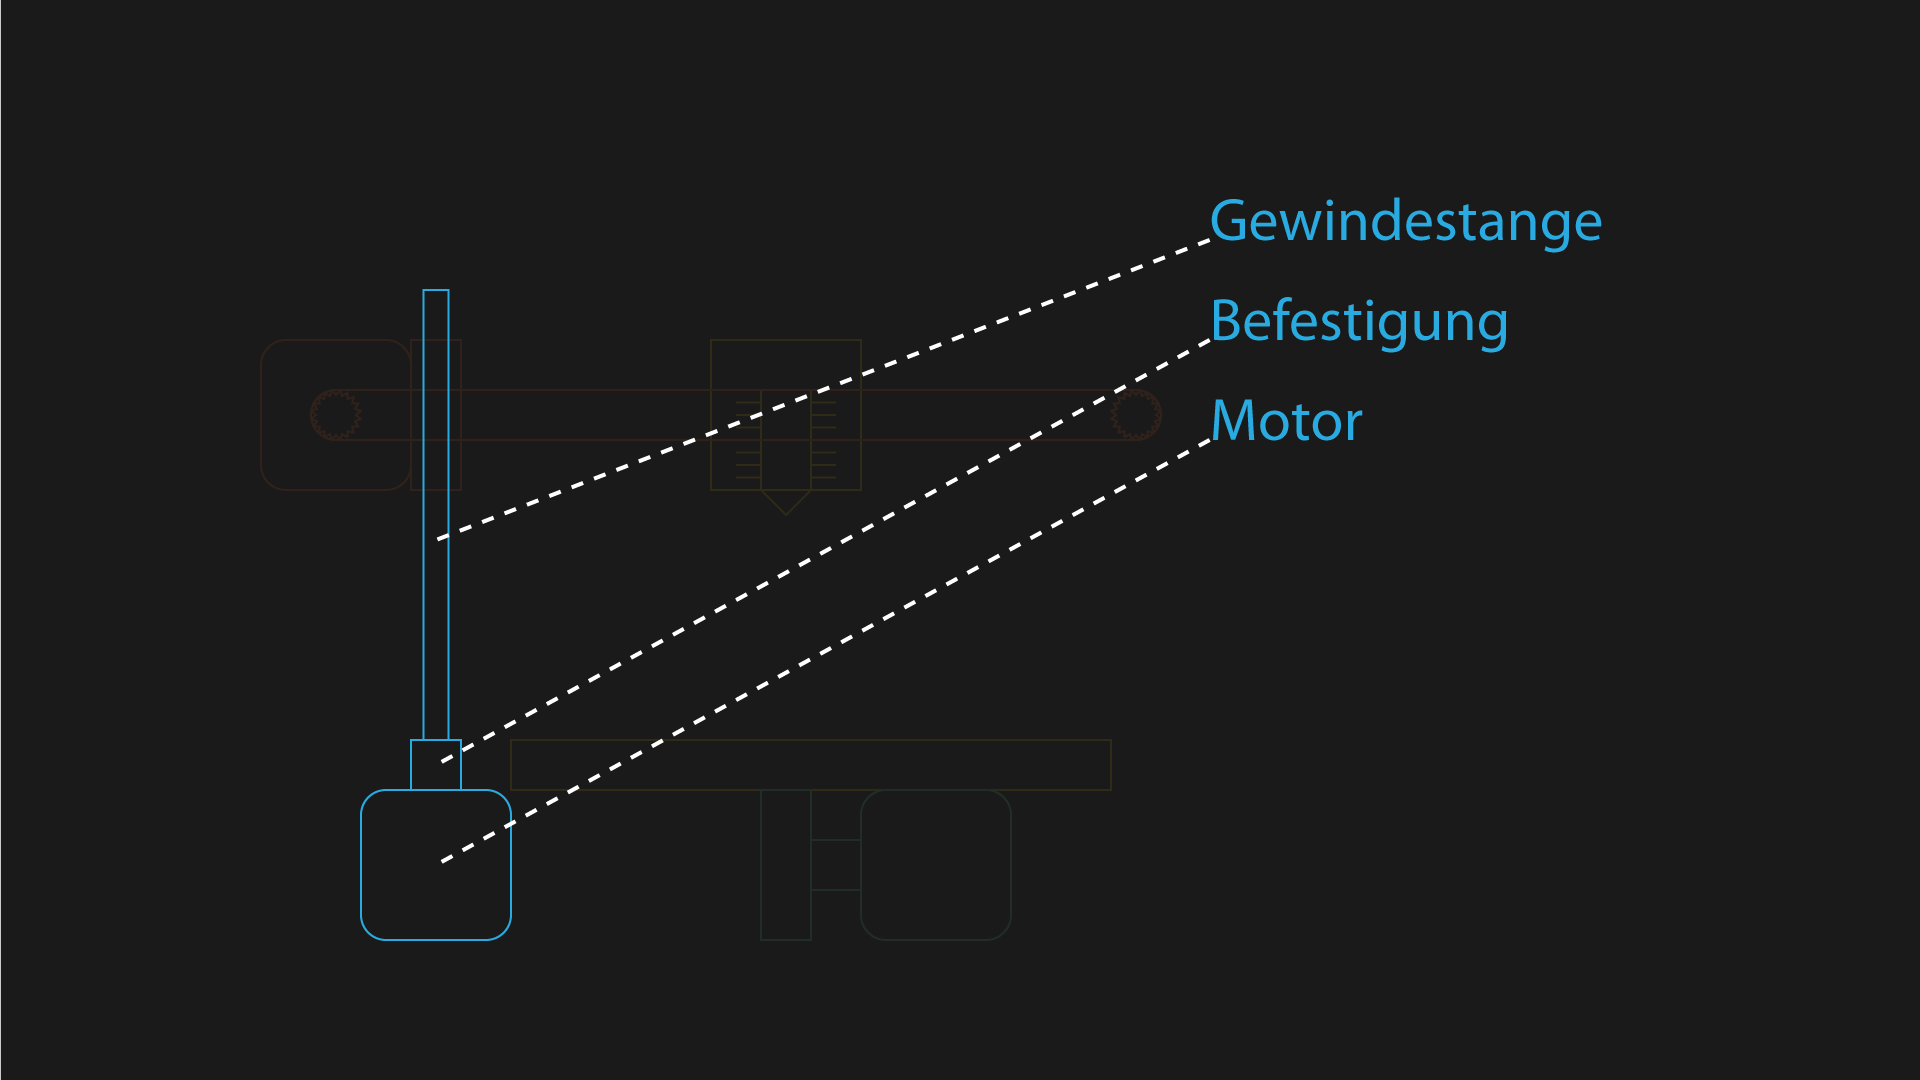
\includegraphics[width=\paperwidth]{images/mechanik/z-axis.png}\hfil}\vfil}
}
}
\begin{frame}
  \frametitle{Z-Achse}
\end{frame}
}

{
\usebackgroundtemplate{%
\colorbox{BackgroundJGH}{%
\vbox to \paperheight{\vfil\hbox to \paperwidth{\hfil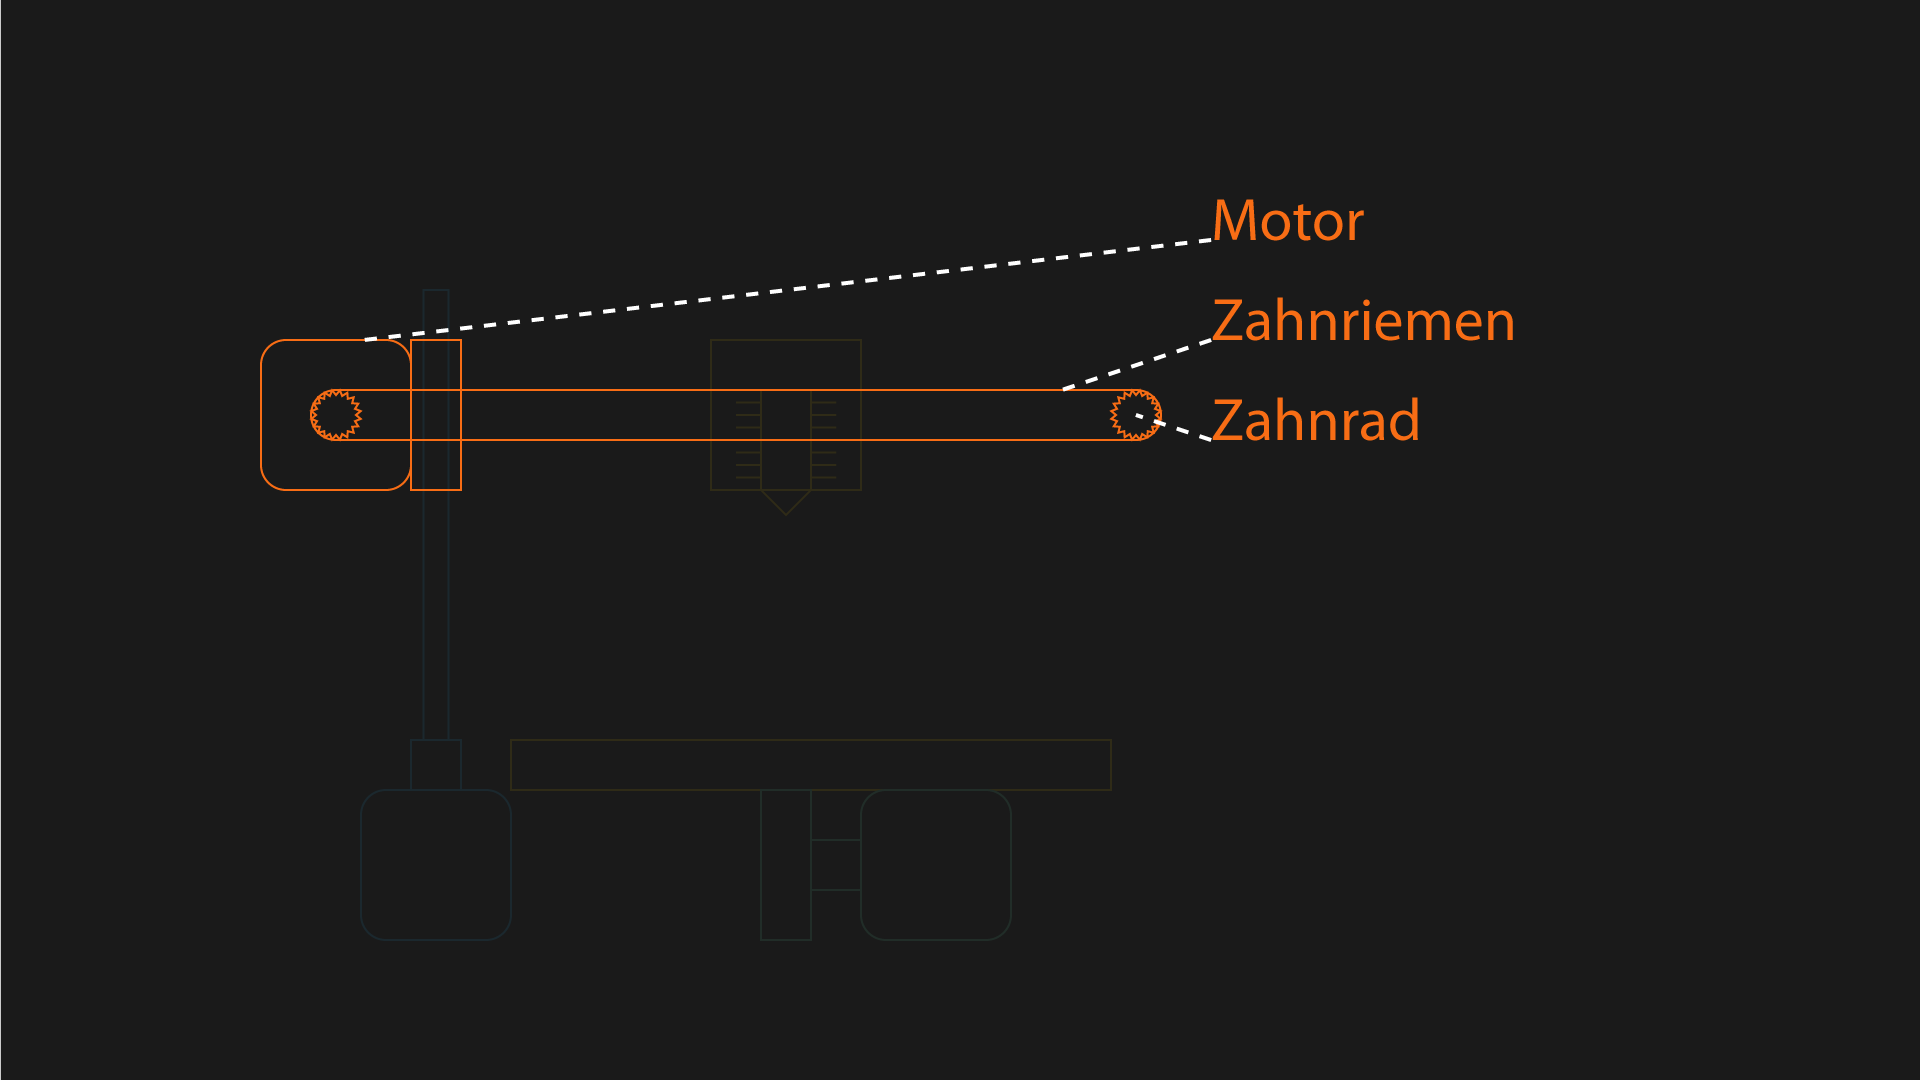
\includegraphics[width=\paperwidth]{images/mechanik/x-axis.png}\hfil}\vfil}
}
}
\begin{frame}
  \frametitle{X-Achse}
\end{frame}
}

{
\usebackgroundtemplate{%
\colorbox{BackgroundJGH}{%
\vbox to \paperheight{\vfil\hbox to \paperwidth{\hfil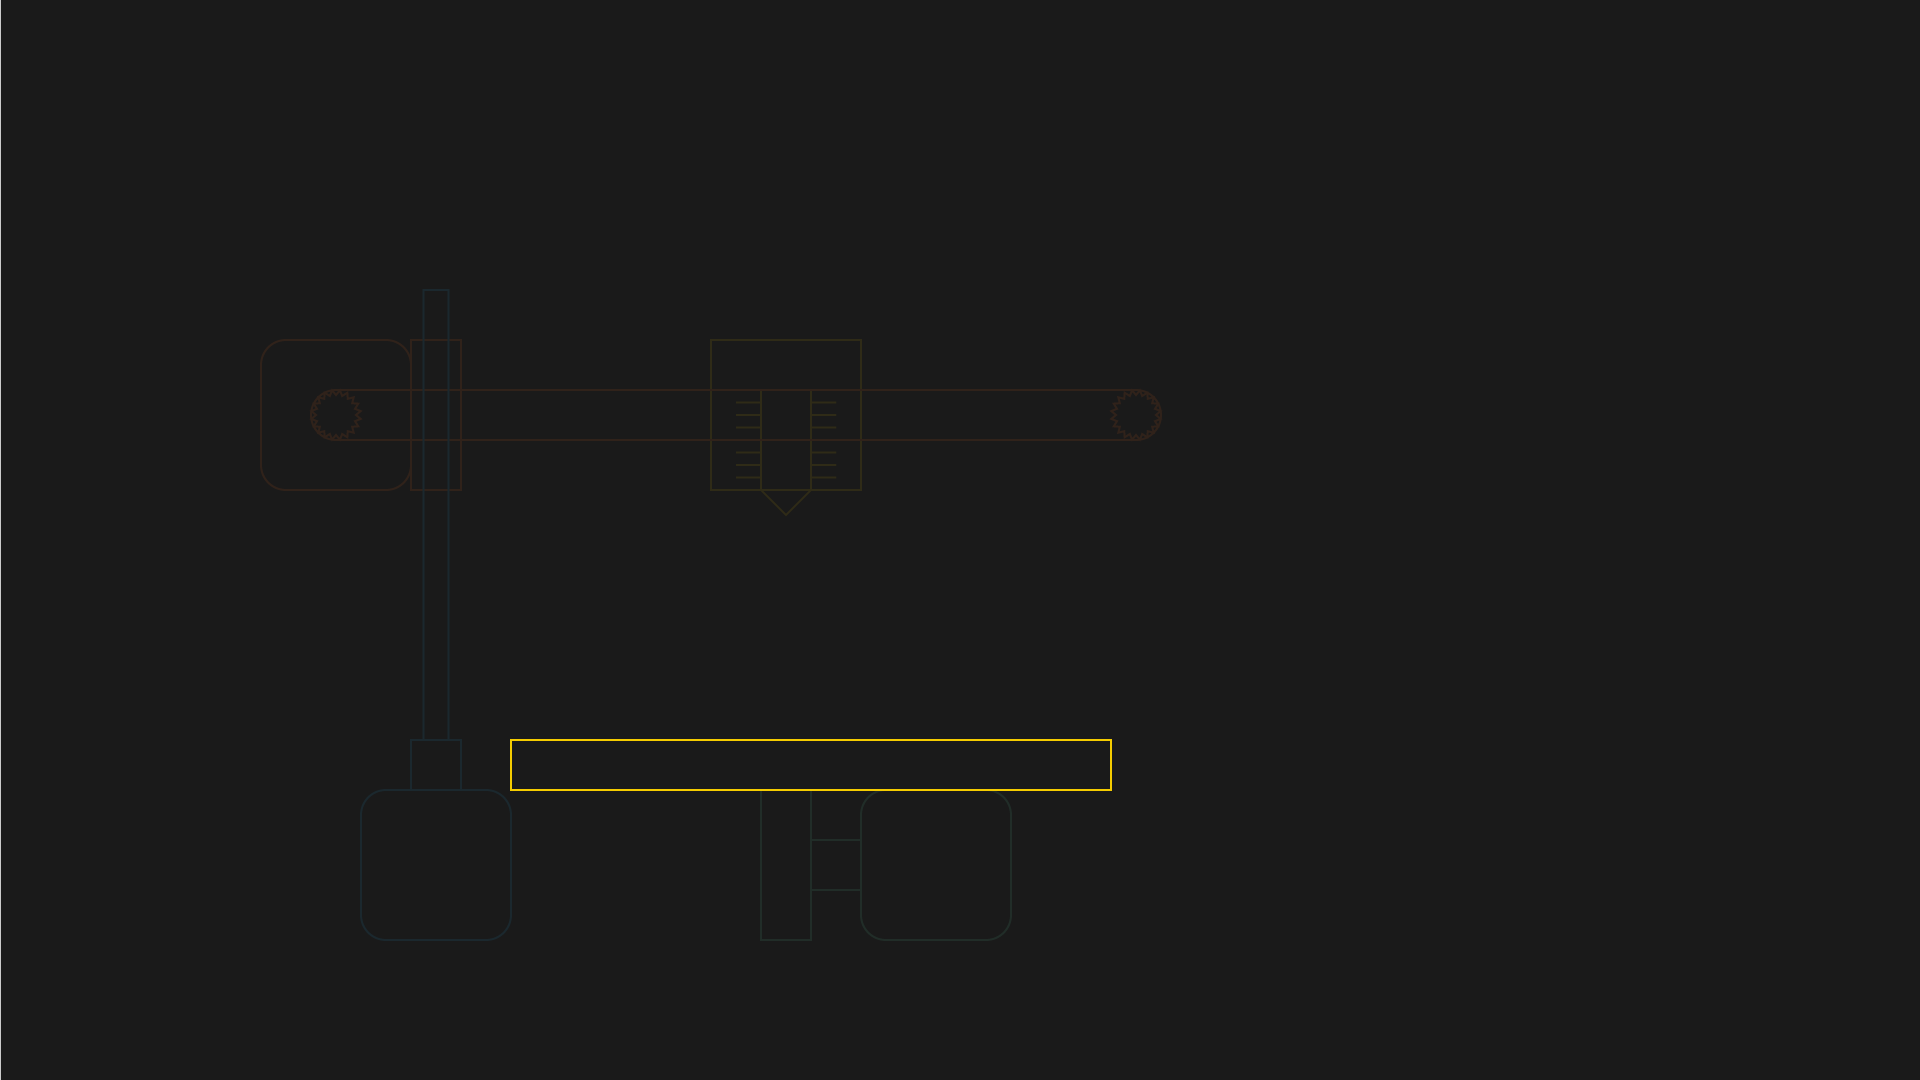
\includegraphics[width=\paperwidth]{images/mechanik/print_bed.png}\hfil}\vfil}
}
}
\begin{frame}
  \frametitle{Druckbett}
  \pause
  \begin{itemize}
    \item Beheizt \pause
    \item Unbeheizt
  \end{itemize}
\end{frame}

\begin{frame}
  \frametitle{Druckbett}
  \begin{itemize}
    \item Glas \pause
    \begin{itemize}
      \item Viele Materialien nur Beheizt
      \item Glastemperatur \pause
    \end{itemize}
    \item Kunststoffe \pause
    \begin{itemize}
      \item Oft mit strukturierter Oberfläche \pause
    \end{itemize}
    \item Bluetape \pause
    \begin{itemize}
      \item Oft zum Verbessern der Haftung verwendet
    \end{itemize}
  \end{itemize}
\end{frame}
}

\subsection{Was ist Filament?}
{
\usebackgroundtemplate{%
\colorbox{BackgroundJGH}{%
\vbox to \paperheight{\vfil\hbox to \paperwidth{\hfil\includegraphics[width=\paperwidth]{images/filament/filament3.jpg}\hfil}\vfil}
}
}
\begin{frame}
  \frametitle{Was ist Filament?} \pause
  \begin{itemize}
    \item Ein Faden aus Thermoplastischem Kunststoff \pause
    \item Je nach Drucker mit verschiedenen Durchmessern \pause
    \item Wird auf einer Spule aufgerollt verkauft
  \end{itemize}
\end{frame}
\begin{frame}
  \frametitle{Physikalische Eigenschaften}
  \pause
  \begin{itemize}
    \item Festigkeit \pause
    \item Flexibilität \pause
    \item Haltbarkeit \pause
    \item Schrumpf und Verzug (Warping) \pause
    \item Löslich (Stützstrukturen)
  \end{itemize}
\end{frame}

\begin{frame}
  \frametitle{Verarbeitungseigenschaften}
  \pause
  \begin{itemize}
    \item Drucktemperatur \pause
    \item Glastemperatur/Druckbett-Temperatur
  \end{itemize}
\end{frame}
}
{
\usebackgroundtemplate{%
\colorbox{BackgroundJGH}{%
\vbox to \paperheight{\vfil\hbox to \paperwidth{\hfil\includegraphics[width=\paperwidth]{images/filament/filament4.jpg}\hfil}\vfil}
}
}
\begin{frame}
  \frametitle{PLA}
  \pause
  \begin{itemize}
    \item Das am häufigsten verwendete Filament \pause
    \begin{itemize}
      \item Biokompatibel
      \item Anwendung in bio Plastiktüten, etc. \pause
    \end{itemize}
    \item Festes, sprödes Material, bricht leicht
  \end{itemize}
\end{frame}

\begin{frame}
  \frametitle{Eigenschaften}
  \pause
  \begin{itemize}
    \item \textbf{Schwierigkeit:} Gering
    \item \textbf{Drucktemperatur:} \unit[180 - 230]{°C}
    \item \textbf{Druckbett-Temperatur:} \unit[20 - 60]{°C}
    \item \textbf{Schrumpf und Verzug:} Gering
    \item \textbf{Haltbarkeit:} Durchschnittlich
    \item \textbf{Glastemperatur:} \unit[45-65]{°C}
    \item \textbf{Löslich:} Nein
  \end{itemize}
\end{frame}

\begin{frame}
  \frametitle{ABS}
  \pause
  \begin{itemize}
    \item Robuster Kunststoff \pause
    \begin{itemize}
      \item Eignet sich zum Beschichten mit Metallen und anderen Kunststoffen
      \item LEGO-Steine, Playmobil, Motorradhelme \pause
    \end{itemize}
    \item Festes, haltbares und temperaturbeständiges Material
  \end{itemize}
\end{frame}

\begin{frame}
  \frametitle{Eigenschaften}
  \pause
  \begin{itemize}
    \item \textbf{Schwierigkeit:} Hoch
    \item \textbf{Drucktemperatur:} \unit[210-250]{°C}
    \item \textbf{Druckbett-Temperatur:} \unit[80 - 110]{°C}
    \item \textbf{Schrumpf und Verzug:} Stark
    \item \textbf{Haltbarkeit:} Hoch
    \item \textbf{Glastemperatur:} \unit[95 - 110]{°C}
    \item \textbf{Löslich:} Ester, Ketonen und Aceton
  \end{itemize}
\end{frame}

\begin{frame}
  \frametitle{PETG}
  \pause
  \begin{itemize}
    \item Lebensmittelsicherheit fraglich (hormonaktive Eigenschaften?) \pause
    \begin{itemize}
      \item Anwendung in PET Flaschen
      \item Teil-biobasiert erhältlich \pause
    \end{itemize}
    \item Festes, flexibles, haltbares Material \pause
    \item Extrem hygroskopisch und klebrig (Stützstrukturen)
  \end{itemize}
\end{frame}

\begin{frame}
  \frametitle{Eigenschaften}
  \pause
  \begin{itemize}
    \item \textbf{Schwierigkeit:} Gering
    \item \textbf{Drucktemperatur:} \unit[220 - 250]{°C}
    \item \textbf{Druckbett-Temperatur:} \unit[50 - 75]{°C}
    \item \textbf{Schrumpf und Verzug:} Gering
    \item \textbf{Haltbarkeit:} Hoch
    \item \textbf{Glastemperatur:} \unit[70]{°C}
    \item \textbf{Löslich:} Nein
  \end{itemize}
\end{frame}

\begin{frame}
  \frametitle{TPU}
  \pause
  \begin{itemize}
    \item Eine Form der Polyurethane \pause
    \begin{itemize}
      \item Anwendung(PU): Schaumstoffe, Lacke, Beschichtungen, Klebstoffe, Vergussmassen
      \item TPU hat fast gummiartige Eigenschaften \pause
    \end{itemize}
    \item Wegen der Materialeigenschaften schwer zu drucken \pause
    \item Extrem hygroskopisch
  \end{itemize}
\end{frame}

\begin{frame}
  \frametitle{Eigenschaften}
  \pause
  \begin{itemize}
    \item \textbf{Schwierigkeit:} Mittel
    \item \textbf{Drucktemperatur:} \unit[210 - 230]{°C}
    \item \textbf{Druckbett-Temperatur:} \unit[30 - 60]{°C}
    \item \textbf{Schrumpf und Verzug:} Gering
    \item \textbf{Haltbarkeit:} Sehr hoch
    \item \textbf{Glastemperatur:} \unit[-223]{°C}
    \item \textbf{Löslich:} Nein
  \end{itemize}
\end{frame}
}

\section{Wie kann ich etwas Drucken?}
{
\usebackgroundtemplate{%
\colorbox{BackgroundJGH}{%
\vbox to \paperheight{\vfil\hbox to \paperwidth{\hfil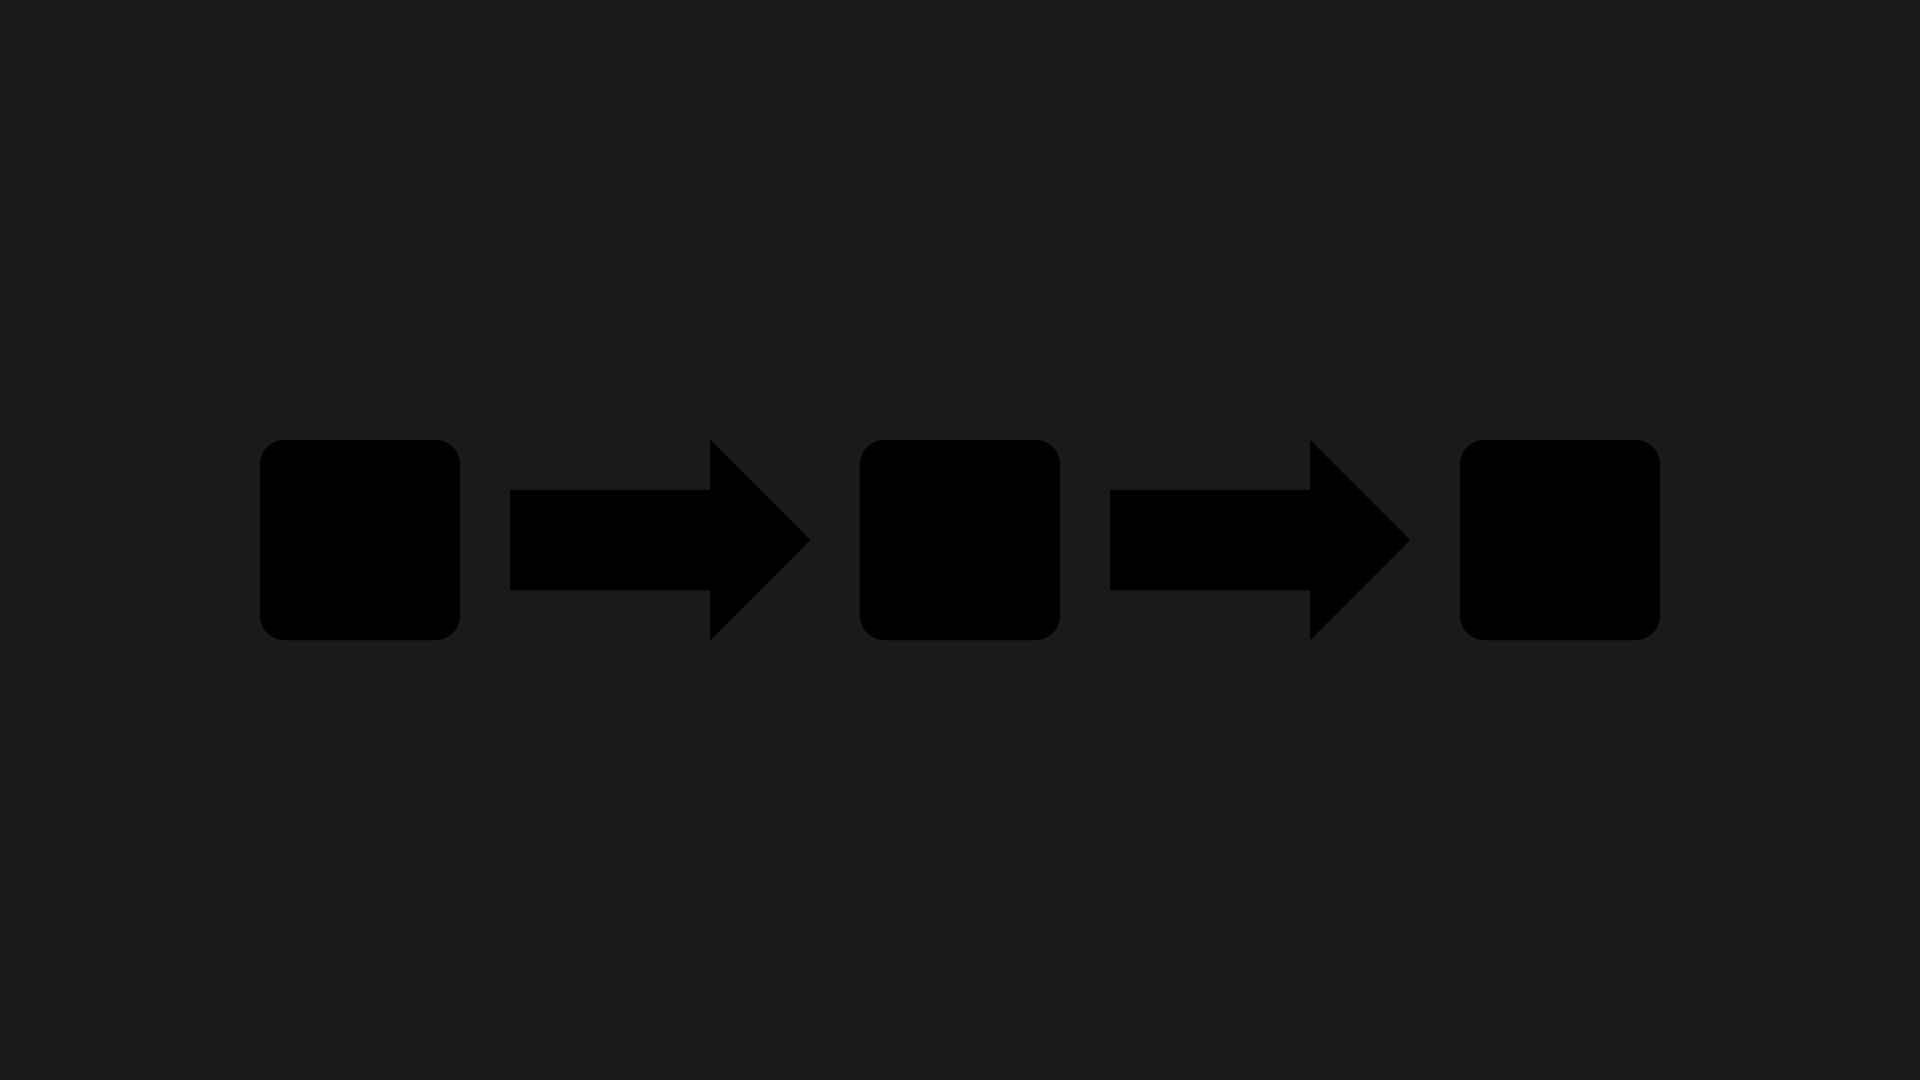
\includegraphics[width=\paperwidth]{images/steps/base.png}\hfil}\vfil}
}
}
\begin{frame}
  \frametitle{Wie kann ich etwas Drucken?}
\end{frame}
}
{
\usebackgroundtemplate{%
\colorbox{BackgroundJGH}{%
\vbox to \paperheight{\vfil\hbox to \paperwidth{\hfil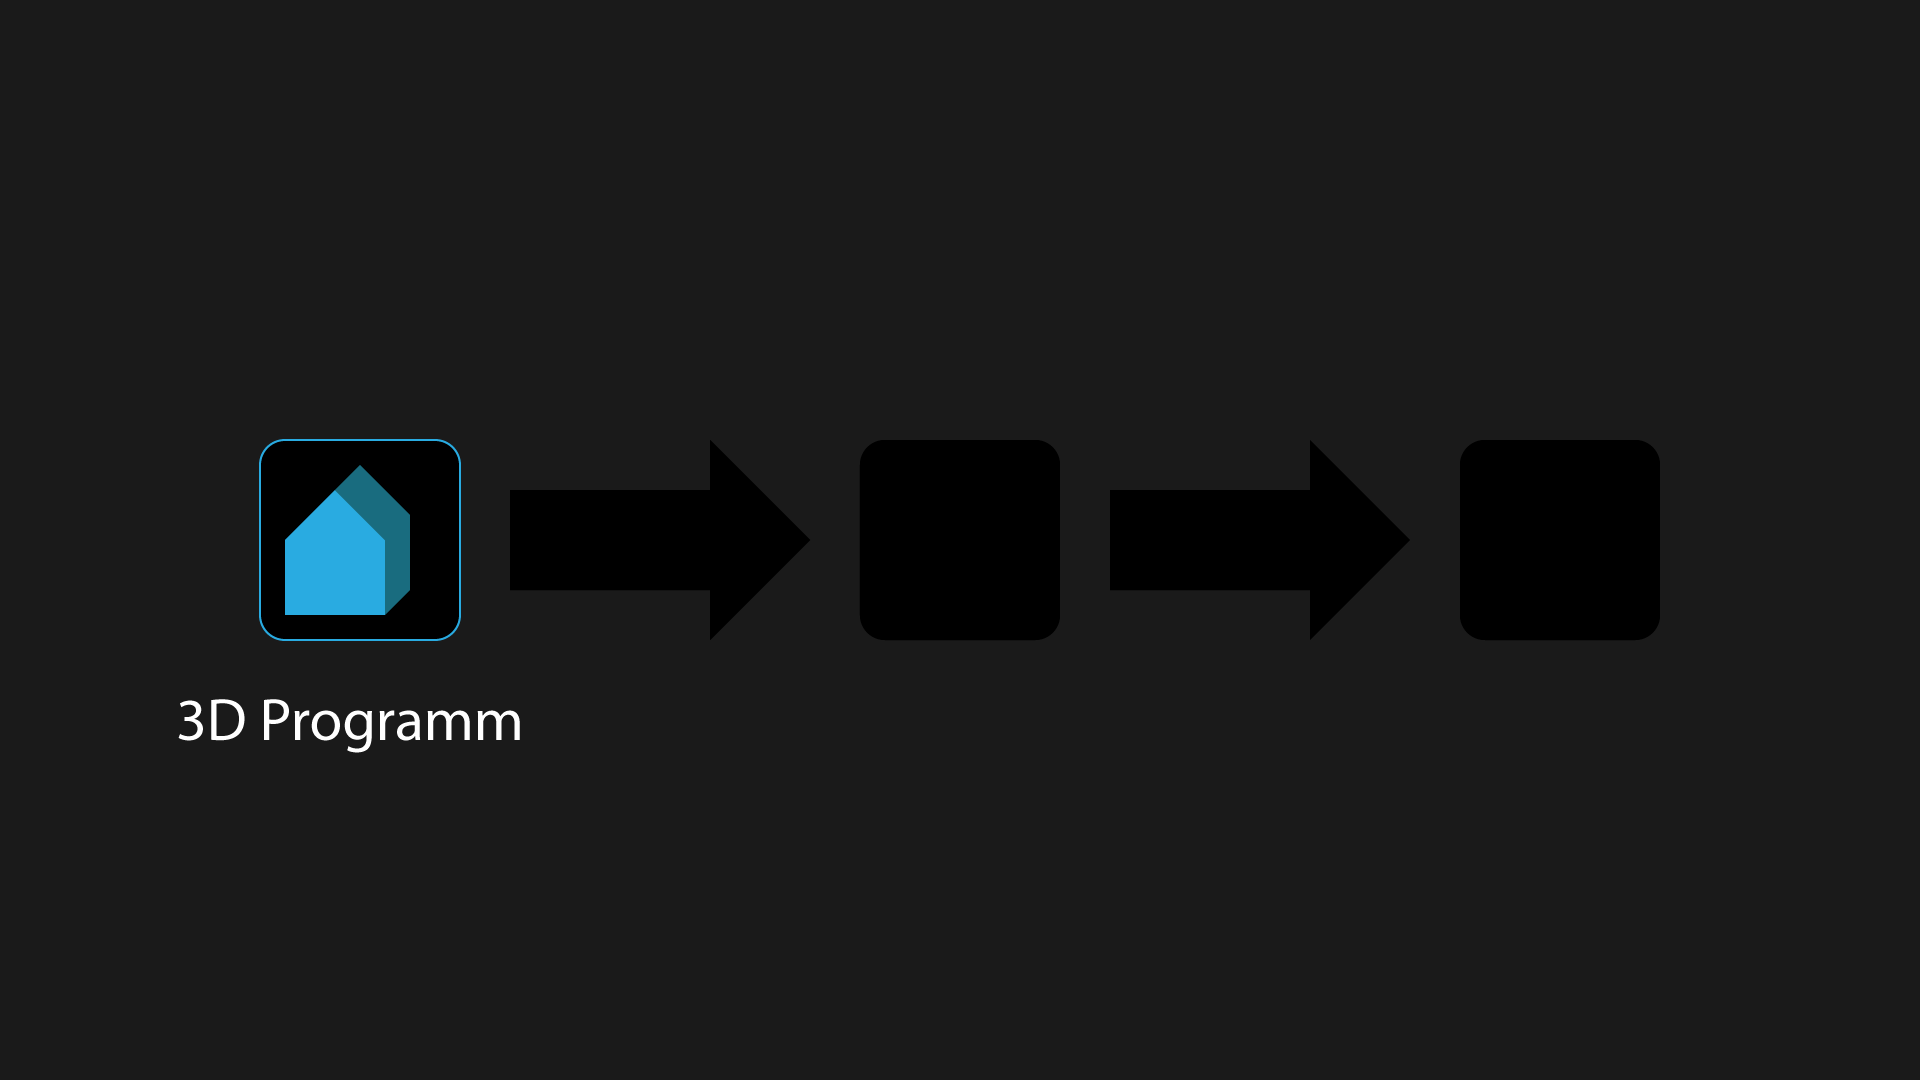
\includegraphics[width=\paperwidth]{images/steps/3d_prog.png}\hfil}\vfil}
}
}
\begin{frame}
  \frametitle{3D Programm}
\end{frame}
}

{
\usebackgroundtemplate{%
\colorbox{BackgroundJGH}{%
\vbox to \paperheight{\vfil\hbox to \paperwidth{\hfil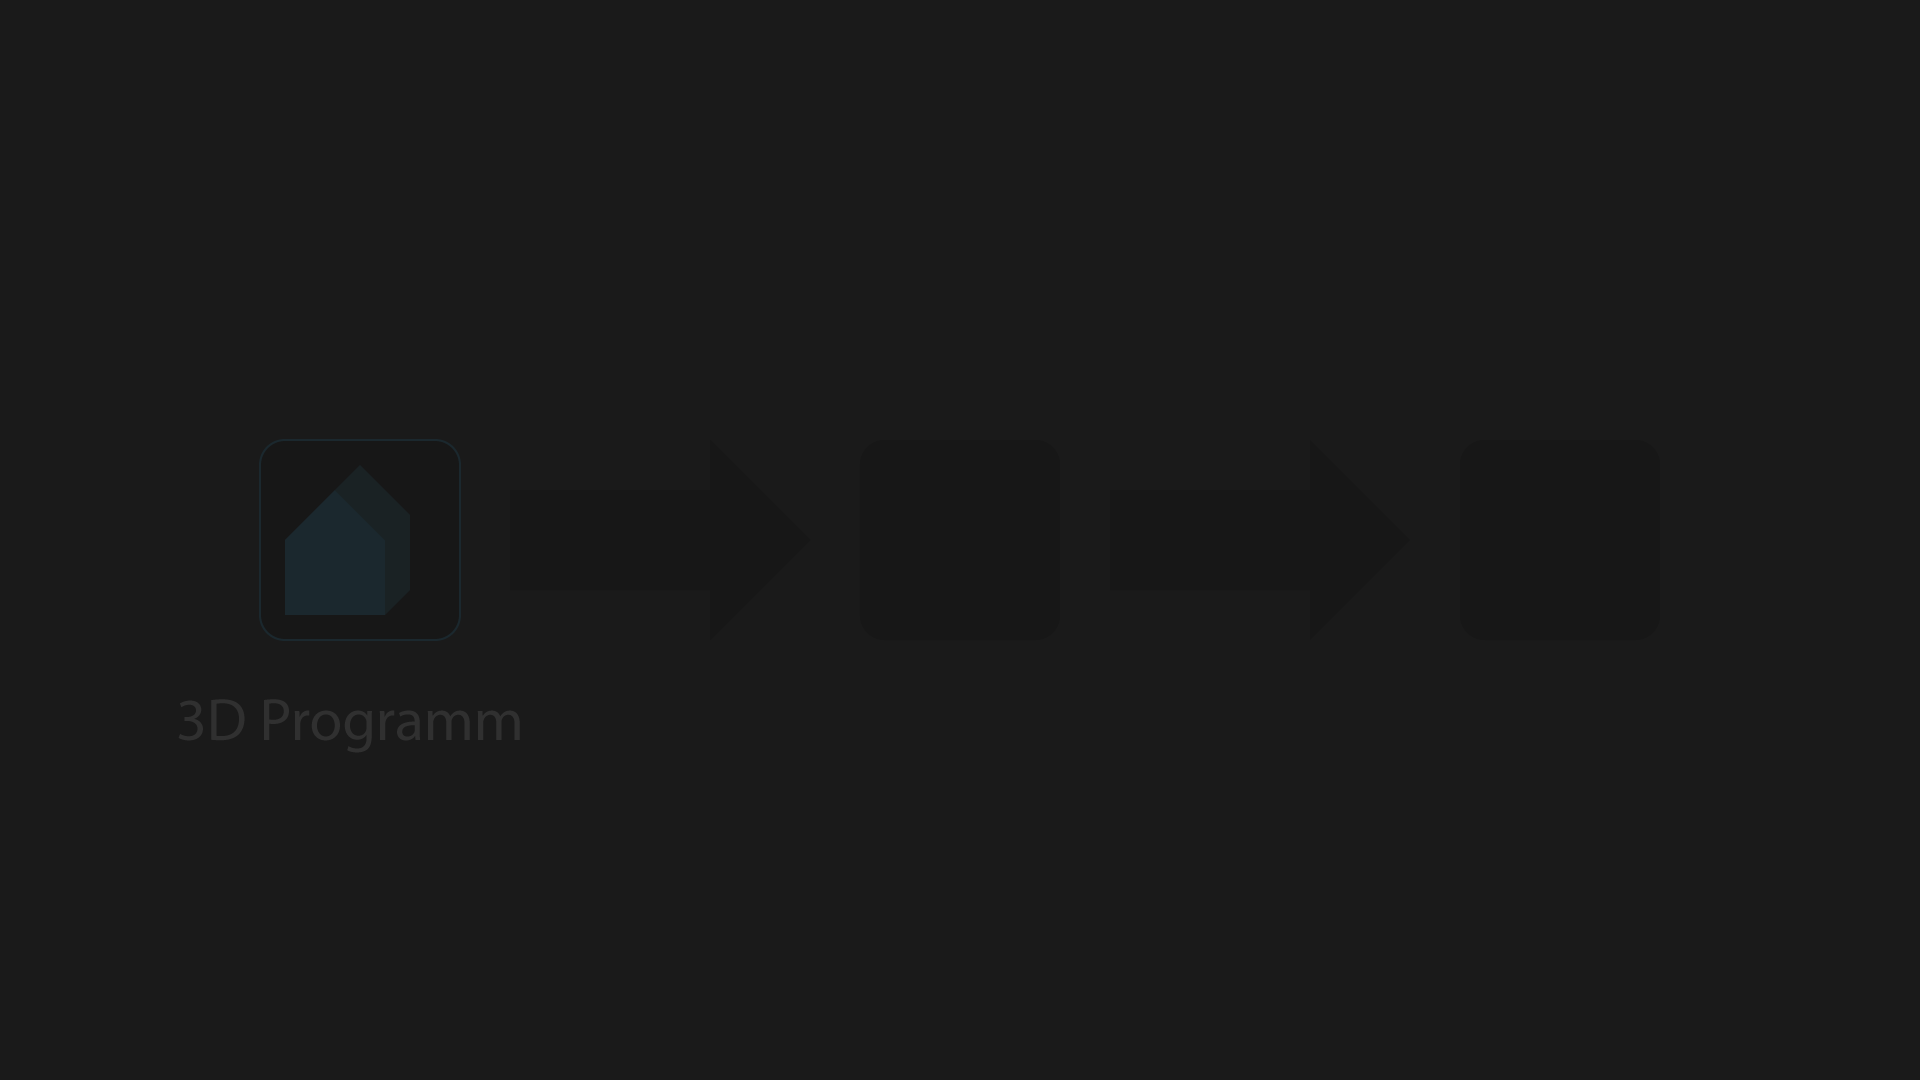
\includegraphics[width=\paperwidth]{images/steps/3d_prog_bg.png}\hfil}\vfil}
}
}
\begin{frame}
  \frametitle{3D Programm}
  \begin{itemize}
    \item Modelierungsprogramm \pause
    \begin{itemize}
      \item Blender \pause
    \end{itemize}
    \item CAD Programm \pause
    \begin{itemize}
      \item FreeCAD \pause
    \end{itemize}
    \item Objektbibliothek \pause
    \begin{itemize}
      \item Thingiverse
    \end{itemize}
  \end{itemize}
\end{frame}
}
{
\usebackgroundtemplate{%
\colorbox{BackgroundJGH}{%
\vbox to \paperheight{\vfil\hbox to \paperwidth{\hfil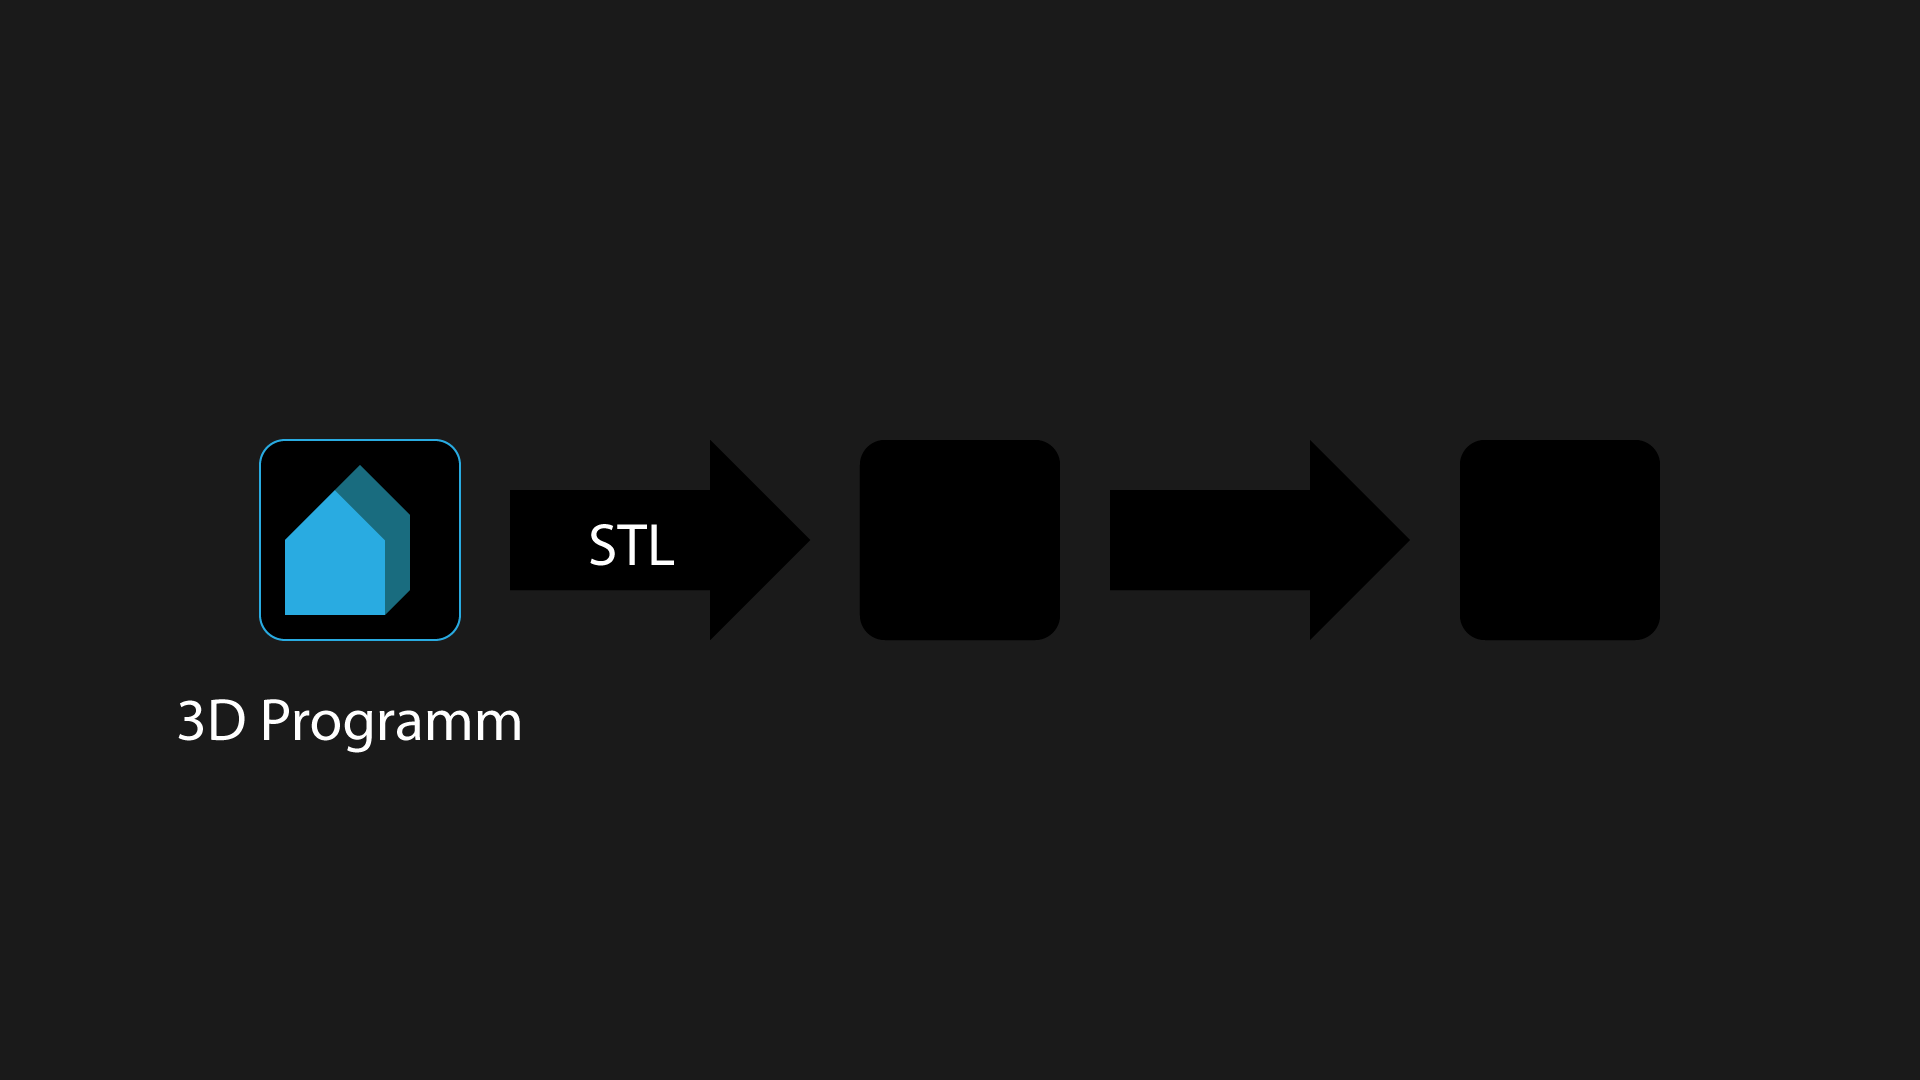
\includegraphics[width=\paperwidth]{images/steps/stl.png}\hfil}\vfil}
}
}
\begin{frame}
  \frametitle{STL Datei}
\end{frame}
}
{
\usebackgroundtemplate{%
\colorbox{BackgroundJGH}{%
\vbox to \paperheight{\vfil\hbox to \paperwidth{\hfil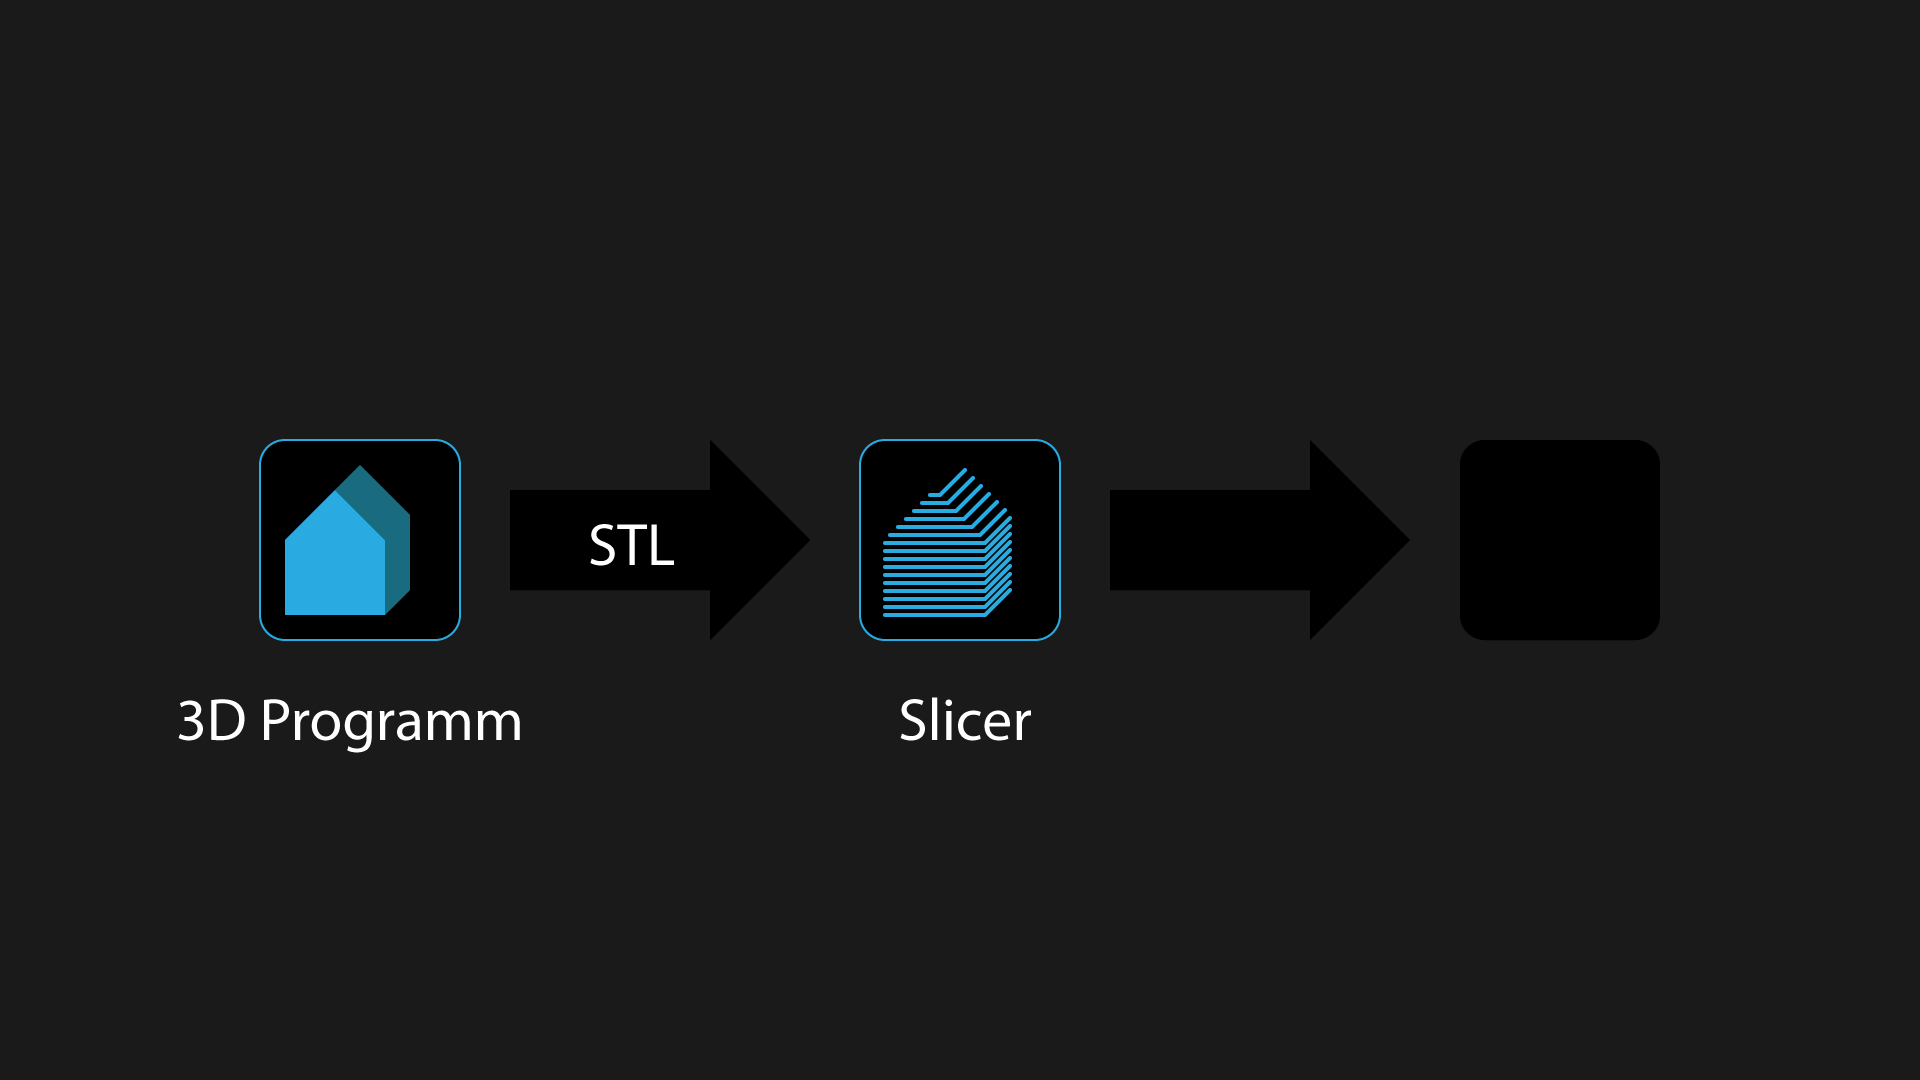
\includegraphics[width=\paperwidth]{images/steps/slicer.png}\hfil}\vfil}
}
}
\begin{frame}
  \frametitle{Slicer}
\end{frame}
}
{
\usebackgroundtemplate{%
\colorbox{BackgroundJGH}{%
\vbox to \paperheight{\vfil\hbox to \paperwidth{\hfil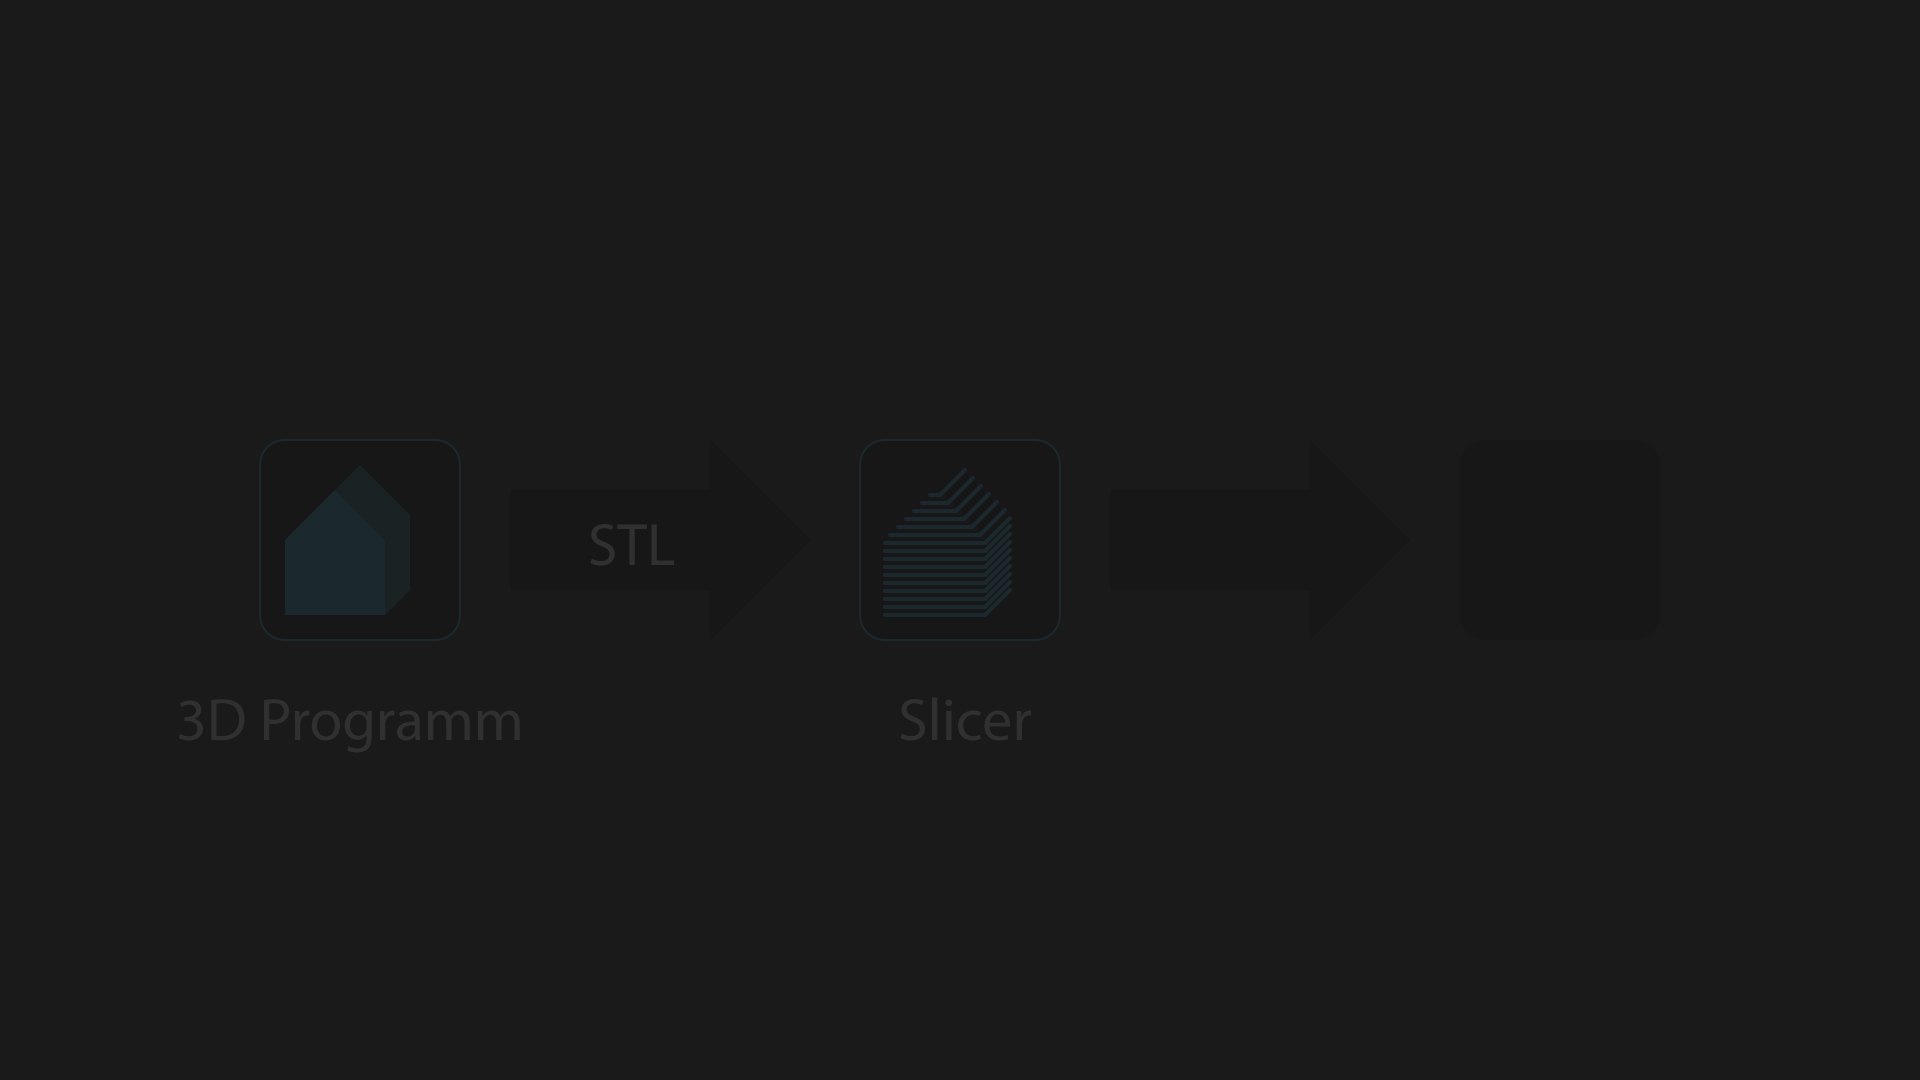
\includegraphics[width=\paperwidth]{images/steps/slicer_bg.png}\hfil}\vfil}
}
}
\begin{frame}
  \frametitle{Slicer}
  \begin{itemize}
    \item Vorbereitung für den Druck \pause
    \begin{itemize}
      \item Auswahl des Druckers \pause
      \item Platzieren auf dem Druckbett \pause
      \item Einstellen der Schichtdicke \pause
      \item Einstellen der Parameter für das Filament \pause
      \item Steuerkommandos für den jeweiligen Drucker
    \end{itemize}
  \end{itemize}
\end{frame}
}
{
\usebackgroundtemplate{%
\colorbox{BackgroundJGH}{%
\vbox to \paperheight{\vfil\hbox to \paperwidth{\hfil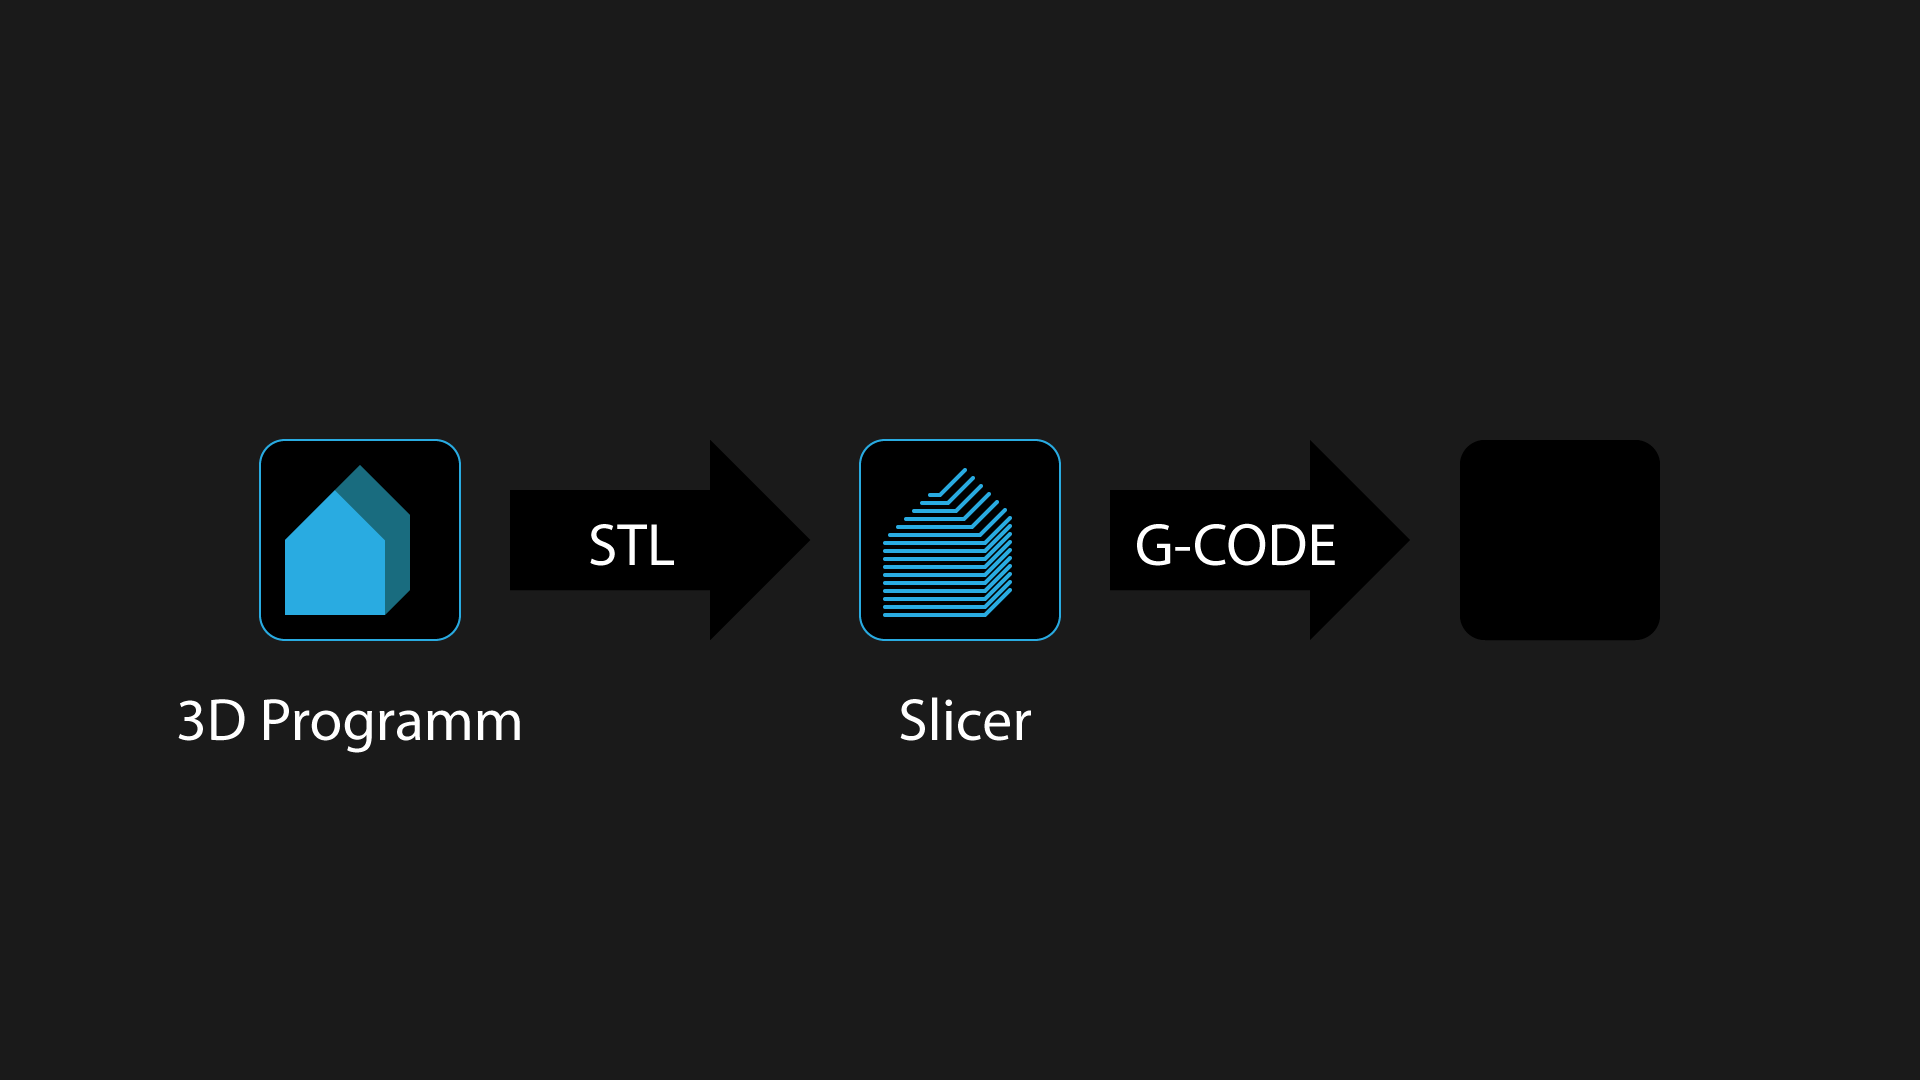
\includegraphics[width=\paperwidth]{images/steps/gcode.png}\hfil}\vfil}
}
}
\begin{frame}
  \frametitle{G-Code Datei}
\end{frame}
}
{
\usebackgroundtemplate{%
\colorbox{BackgroundJGH}{%
\vbox to \paperheight{\vfil\hbox to \paperwidth{\hfil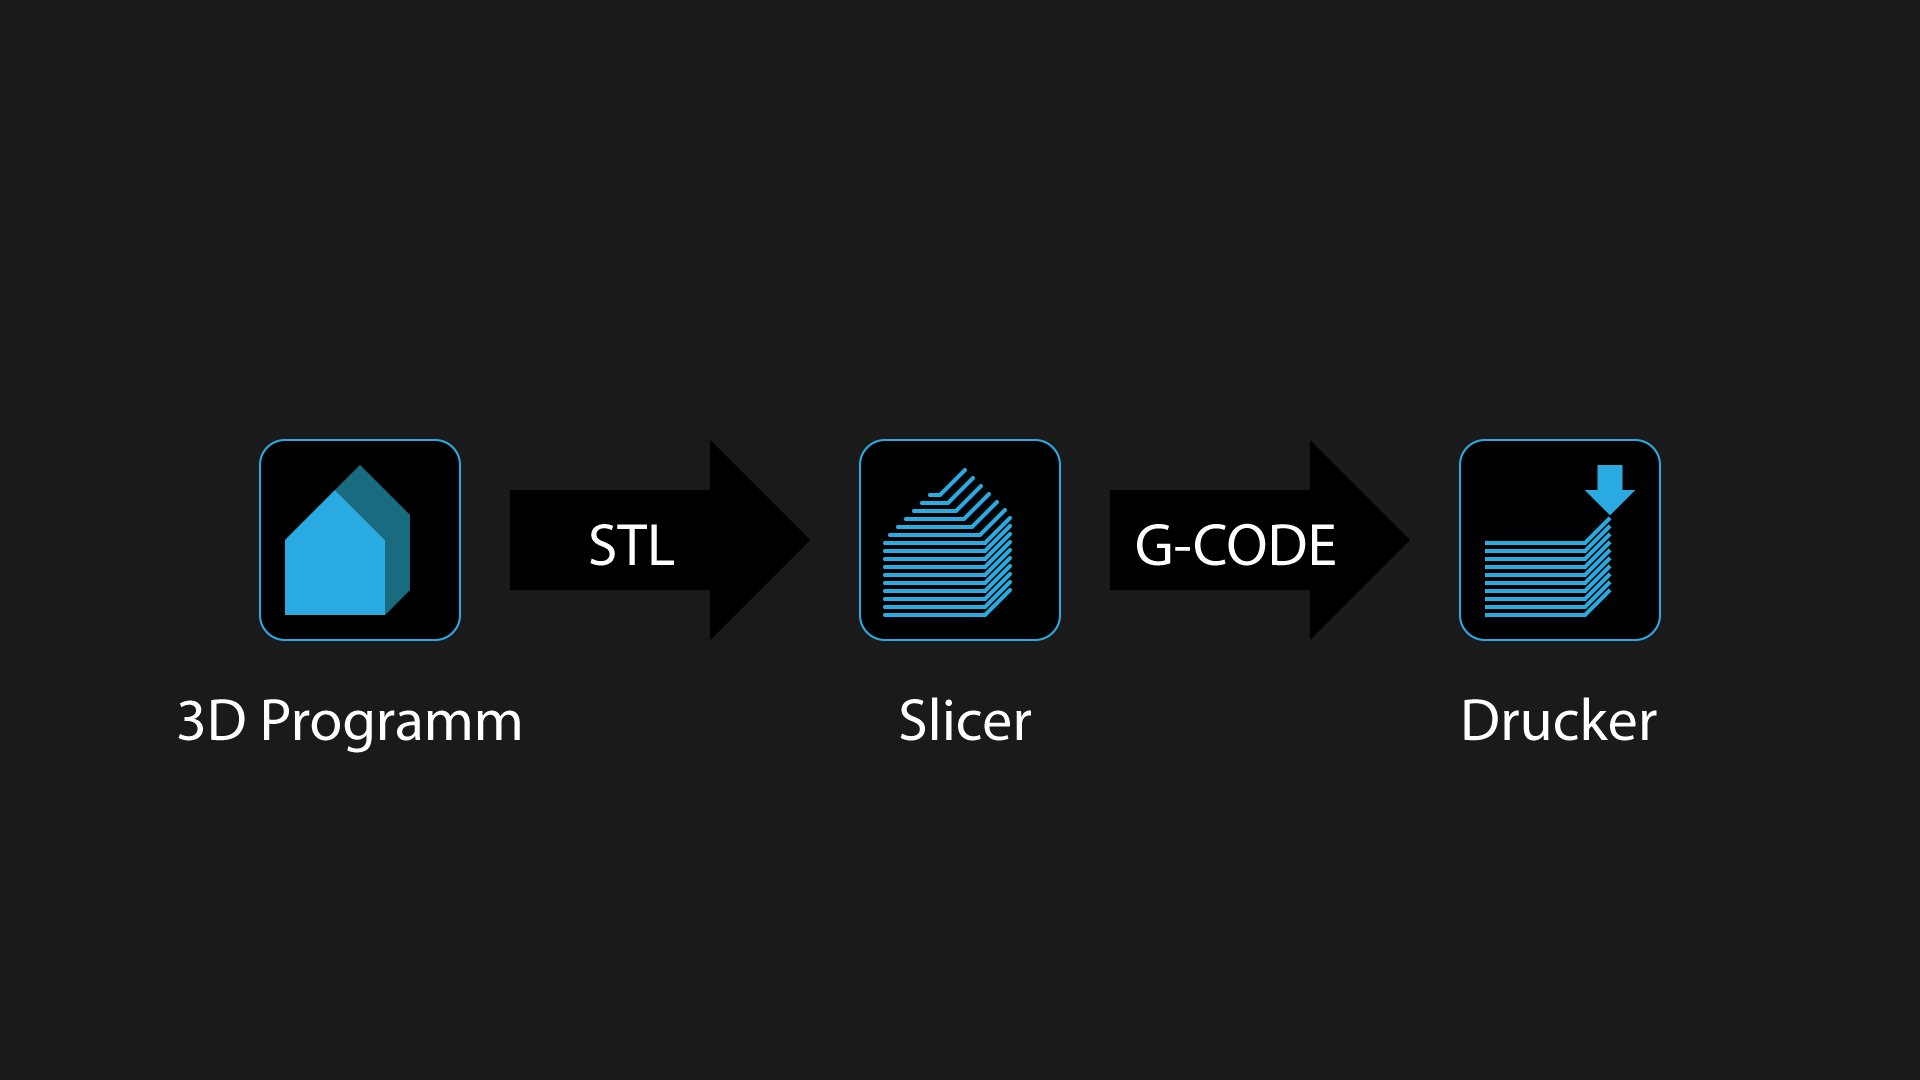
\includegraphics[width=\paperwidth]{images/steps/drucker.png}\hfil}\vfil}
}
}
\begin{frame}
  \frametitle{Drucker}
\end{frame}
}
{
\usebackgroundtemplate{%
\colorbox{BackgroundJGH}{%
\vbox to \paperheight{\vfil\hbox to \paperwidth{\hfil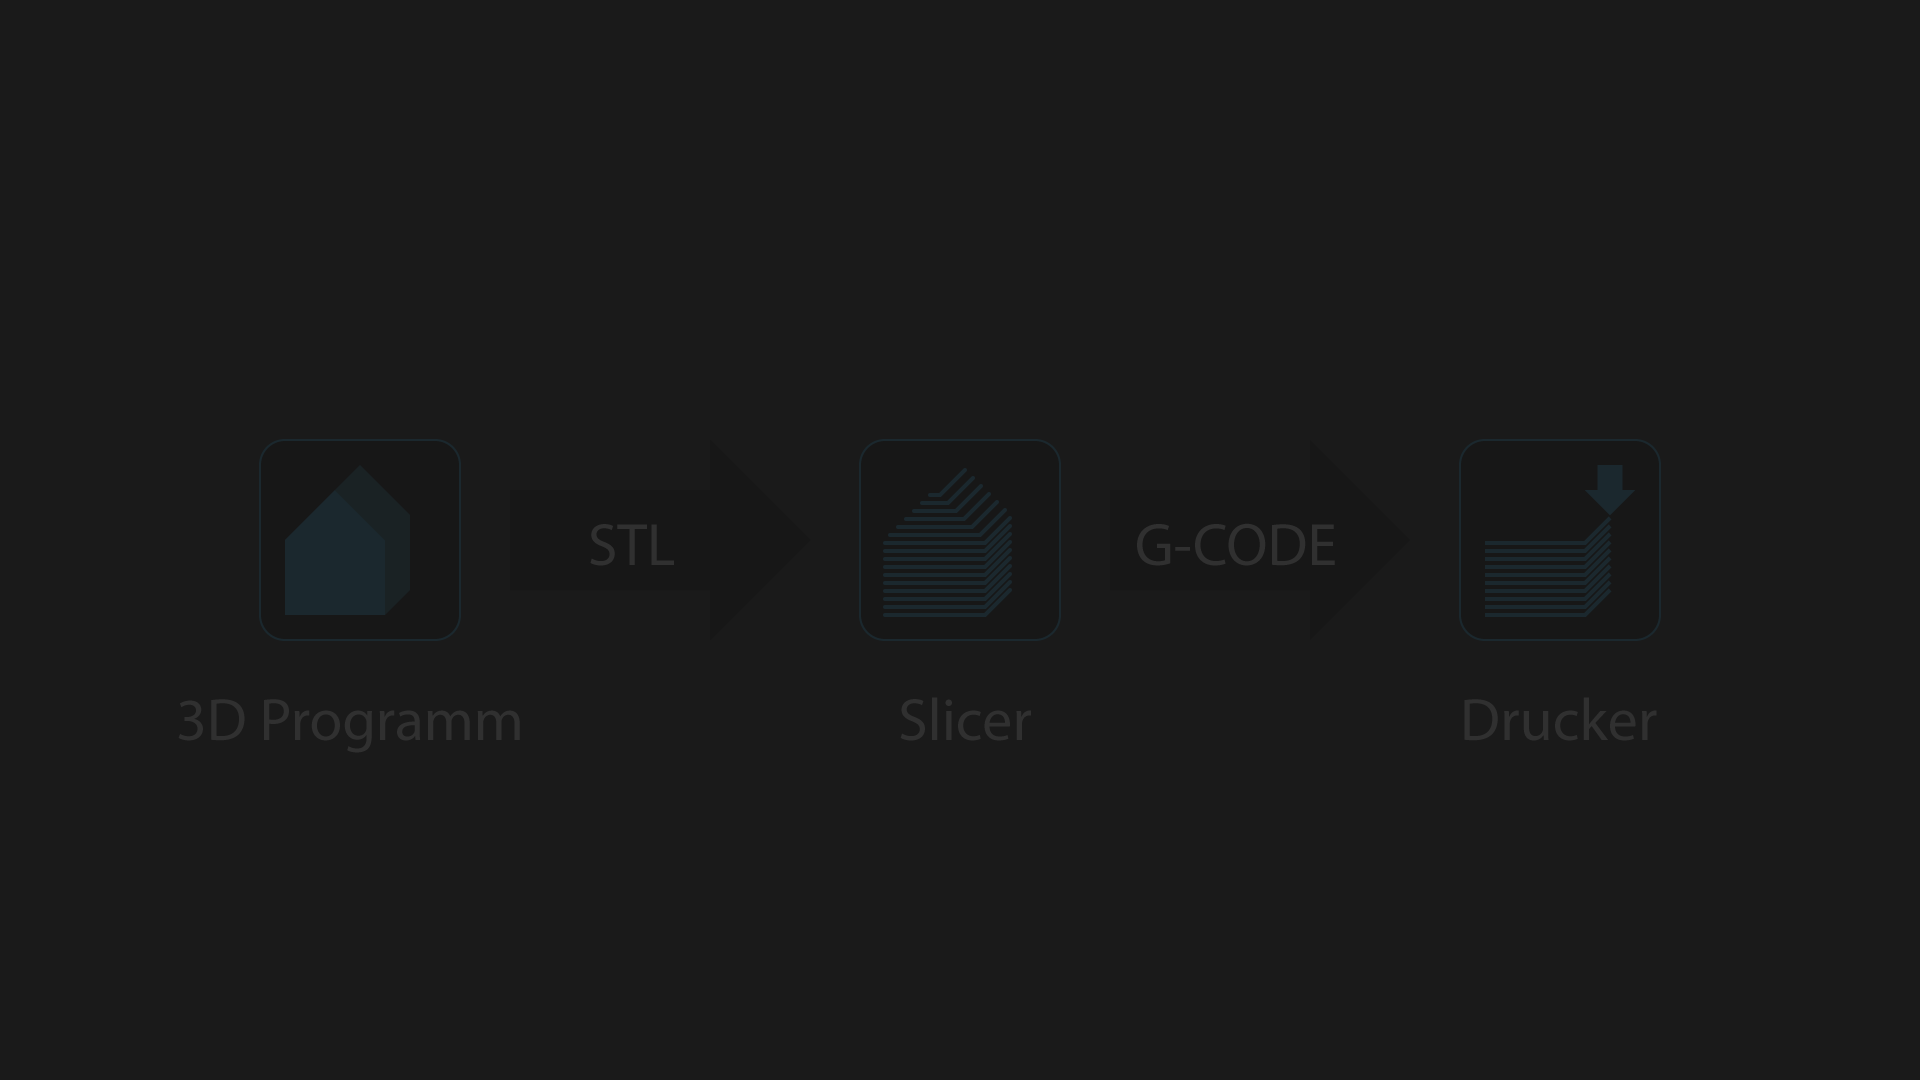
\includegraphics[width=\paperwidth]{images/steps/drucker_bg.png}\hfil}\vfil}
}
}
\begin{frame}
  \frametitle{Drucker}
  \begin{itemize}
    \item Übertragen der G-Code Datei \pause
    \begin{itemize}
      \item SD-Karte \pause
      \item USB-Stick \pause
      \item WiFi \pause
    \end{itemize}
    \item G-Code nur mit jeweiligem Drucker kompatibel \pause
    \begin{itemize}
      \item Vorsicht! Drucker kann kaputt gehen!
    \end{itemize}
  \end{itemize}
\end{frame}
}


\end{document}
